%!TEX root = ../thesis.tex
%*******************************************************************************
%****************************** Third Chapter **********************************
%*******************************************************************************
\chapter{Experimental Work}

% **************************** Define Graphics Path **************************
\ifpdf
    \graphicspath{{Chapter6/Figs/Raster/}{Chapter6/Figs/PDF/}{Chapter6/Figs/}}
\else
    \graphicspath{{Chapter6/Figs/Vector/}{Chapter6/Figs/}}
\fi

\section{Introduction}
\subsection{Background}
Diamond offers unique material properties for electrical devices that are unparalleled by other wide bandgap semiconductors. In the creation of devices that rely upon n and p-type doping however, many challenges arise from the limitations that diamond imposes upon device fabrication. Due to its extraordinary hardness and densely packed crystal lattice, doping via implantation has had marginal success and CVD growth is the preferred choice for doped material. The selection of donor candidates is limited, with nitrogen forming a deep donor level of around 1.6--1.7 \si{\electronvolt} [\cite{li1998}] due to a chemical re-bonding of the donor electron on a neighbouring carbon atom simultaneous with a lone-pair on the nitrogen atom itself [\cite{goss2008}]. Phosphorous, despite having a lower solubility than nitrogen within the diamond lattice, is able to provide a shallower donor level at around 0.57--0.60 \si{\electronvolt} [\cite{koizumi2000}]. Various strategies of co-doping phosphorous with other elements have been examined theoretically such as in \cite{alfieri2018}, but experimentally, substitutional phosphorous remains the only practical n-type donor within diamond. The maximum dopant concentration depends primarily on the crystal orientation, with the \hkl{111} orientation providing the highest observed concentrations of around $1\times10^{20}$ \si{\atoms\per\centi\metre\cubed} [\cite{grotjohn2014}. Boron doped p-type material is most readily deposited onto the \hkl{100} orientation, in large part due to the ready incorporation of crystalline defects on the \hkl{111} orientation. Typical Hall mobility measurements for boron doped diamond at room temperature on \hkl{111} oriented samples are around 500 \si{\cm\squared\per\volt\per\second} as seen in \cite{ri2005} while on \hkl{100} oriented samples the Hall carrier mobility reaches 2000 \si{\cm\squared\per\volt\per\second} as demonstrated by \cite{mortet2008}. These defects in \hkl{111} oriented diamond growth have led to significant efforts in the improvement of \hkl{100} oriented phosphorous doped CVD growth, with concentrations in the range of $10^{16}-10^{18}$ [\cite{kato2007}]. However, high compensation ratios become a significant limiting factor in phosphorous doped films grown on \hkl{100} oriented substrates as investigated more recently by \cite{stenger2021}.

\subsection{Ohmic Contact Formation to Diamond Devices}
One common theme throughout the development of diamond based electronic devices is the challenge of ohmic contact formation, as well as reliable Schottky contacts. This is in large part due to the presence of significant charge screening, resulting in strong Fermi level pinning at the diamond surface in both boron [\cite{baker1993}] and phosphorous [\cite{suzuki2006}] doped samples. This is a significant issue for devices that require phosphorous doped diamond, due to the significant activation energy required for carrier promotion. While boron doped diamond can reach a metallic level at around $10^{20}$ \si{\atoms\per\centi\metre\cubed}, allowing for high quality ohmic contact formation via annealed titanium with standard capping layers of gold or platinum/gold, this is not the case for phosphorous doping. This can be expressed with the ideal theory of metal to n-type semiconductor contacts, in which the contact resistivity $\rho_{c}$ varies exponentially by the factor $\frac{\phi_{b}}{\sqrt{N_{D}}}$ where $\phi_{b}$ is the Schottky barrier height and $N_{D}$ is the active donor concentration. Since it is difficult to deviate from the Fermi level pinning of $\approx4.3$ \si{\electronvolt} below the conduction band, instead the approach to reduce contact resistivity is to increase the doping concentration $N_{D}$. This has previously been used to great effect in boron doped diamond, where the Fermi level pinning of oxygen terminated diamond relative to the valence band is around $1.3$ \si{\electronvolt} [\cite{yamanaka2000}] and has the same issues with regards to the independence of Schottky barrier height from metal contact work functions. With boron doping of $2\text{\textendash}6\times10^{17}$ \si{\atoms\per\centi\metre\cubed}, specific contact resistances of $1.3\times10^{-5}$ \si{\ohm\centi\metre\squared} have been demonstrated using annealed Ti contacts [\cite{chen2005}].

%Ushizawa1998 compared boron growth of 100 and 111 - 111 better for high boron dopant? higher concentration on 111 anyway - preferential growth in high boron conditions. same for phosphorous then? only the crystalline quality that might be a massive factor for 100 samples versus 111 but also we don't need such high concentrations of boron so I guess 10^19 on 100 is more than enough lol. Only an issue for my deep trap 0.6ev phosphorous.... large differences in the growth mechanism too, high methane produces better samples on 111 - ri2005, opposite for 10? 
\subsection{Overview of Methodology and Novel Techniques}
In this chapter, various experimental characterisation methods have been employed to investigate the properties of heavily phosphorous doped diamond as used in ohmic contact fabrication. Recent efforts such as that of \cite{abubakr2022} in laser-induced ohmic contact formation for diamond detector charge collectors and \cite{valappil2023} in corrosion-resistive coaxial arc plasma deposited nanocarbon electrodes clearly demonstrate the ongoing development of phosphorous based devices, with a heavy focus on new methods for forming ohmic contacts in various device structures.

Through standard photolithography and metal deposition, simple Ti/Au and Ti/Pt/Au contacts were investigated and studied across a wide range of temperatures. Differences in the annealing conditions as well as the quality of the photolithography resulted in quite different experimental observations for this material. To understand the possible causes of some of these differences, other material characterisation methods are performed to help elucidate on the nature of heavily phosphorous doped diamond such as SIMS, XPS, AFM and optical microscopy.

Then, another avenue to improve the characteristics of ohmic contacts to heavily phosphorous doped diamond is explored, that of ohmic contacts formed via laser graphitisation of the surface. Further material characterisation techniques such as PL combined with the previous data provides an intriguing picture of laser graphitised phosphorous doped diamond. In particular, the transition from standard Schottky thermionic emission to Fowler-Nordheim type field effect emission via geometric field enhancement is examined, with a consideration of potential cold cathode style devices that could be fabricated via this material and related fabrication techniques. This is in contrast to contact roughening techniques such as that demonstrated in \cite{temahuki2017}, where Ni-catalysed micro-pyramidal \hkl{111} structures are etched into \hkl{100} diamond samples and then overgrown with highly phosphorous doped diamond.

\begin{table}[h]
\centering
\caption{A summary of all \hkl{111} samples, which had differing thicknesses of heavily phosphorous doped surface layers grown via MPCVD at Evince technology. Indicated in the table, various characterisation techniques are used to examine the phosphorous doped diamond and the resulting electrical contacts used in each case.}
\label{table:samples_summary}
\begin{tabular}{|c|c|c|c|c|}

\hline
Sample & Batch & Thickness (\si{\micro\metre}) & Contacts & Characterisation \\
\hline
A & 1 & 0.3 & None & SIMS \\
B & 1 & 0.3 & None & SIMS \\
C & 2 & 0.3 & Ti/Pt/Au - 850\si{\degreeCelsius} 30 mins  & TLM, AFM \\
D & 2 & 0.3 & Ti/Pt/Au - 600\si{\degreeCelsius} 300 mins & TLM, AFM \\
E & 3 & 1.2 & None & XPS \\
F & 3 & 1.2 & Ti/Au - 500\si{\degreeCelsius} 10 mins     & TLM, AFM, HIM \\
G & 3 & 1.2 & Laser Graphitised                          & TLM, AFM, FL \\
% Add more samples here
\hline
\end{tabular}
\end{table}

The samples examined in this chapter are summarised in table \ref{table:samples_summary}. One significant consideration in comparing results from different samples is that the growth of defect-laden phosphorous doped diamond on differing HPHT substrates may incur some loss of similarity between different samples, even when grown in the same batches. This is partially due to the process of microwave plasma CVD growth itself, multiple samples within the growth chamber will necessarily be situated in differing locations within the plasma. Hence, it is impossible to assume complete consistency between differing samples, despite best efforts to ensure these comparisons are comparable.

\section{Sample Preparation}
Examples of (111) HPHT samples are shown in figure \ref{fig:111_samples}. All samples ranged from 1.5--2.5 \si{\milli\metre\squared}, with differing (111) polished faces based on the exact cut of the samples. The literature for diamond surface preparation displays a rich evolution of methods tailored to the unique demands of semiconductor surface treatments. Foundational studies, such as that by \cite{baral1996}, explored a plethora of cleaning procedures, including the use of sulphuric acid-ammonium persulphate and hydrogen plasma. Yet, these procedures have since lost prominence in the literature, suggesting the rapid development and optimisation in the field.

\begin{figure}[h]
\centering
\includegraphics[width=\textwidth]{samples from 2019 - upscaled.png}
\caption{HPHT (111) samples as provided by Element Six, prior to cleaning and deposition.}
\label{fig:111_samples}
\end{figure}

Modern techniques have predominantly converged around variations of dual or tri-acid treatments. \cite{koizumi2000}, \cite{teraji2000,teraji2003}, and \cite{kociniewski2006,kociniewski2007}, for instance, have favoured a triacid mix of \ce{H2SO4}:\ce{HNO3}:\ce{HClO4}, albeit at different ratios and durations. Some researchers such as \cite{kato2005,kato2009} and \cite{suzuki2004}, however, have leaned towards dual acid organic cleans, utilising \ce{H2SO4} and \ce{H2O2} or \ce{H2SO4} and \ce{HNO3}. 

The various methods of surface preparation underscores the importance of optimising cleaning conditions to the specifics of the application in question. Evince technology employed the following standard surface preparation, with a strong focus on ensuring the removal of graphitic carbon and the formation of a consistent oxygen surface termination prior to phosphorous doped CVD growth, and as such this was used for the work in this project:

\subsubsection{Decon90/ Deionised (DI) Water - 5 minutes.}
This acts as an initial cleaning step to remove gross contamination, including organic and inorganic residues. It provides a good general cleaning step that removes common contaminants from the sample surface, especially with a sonication bath providing agitation of the submersed samples. 

\subsubsection{DI Rinse and Sonication - 5 minutes.}
Rinsing the samples with deionised water and sonicating them to ensure complete removal of the initial Decon90 solution, along with any remaining contaminants. Thorough rinsing is crucial to prevent any residues from the first cleaning step, which might interfere with subsequent processes, especially the chemical reactions in the following cleaning stages.

\subsubsection{1:1 \ce{H2SO4} and \ce{H2O2} Mix - 25 minutes at 175\si{\degreeCelsius}.}
This step employs a "piranha solution," a mixture of \ce{H2SO4} and \ce{H2O2}, to further remove organic residues and contaminants. The strong oxidising nature of this mix at the specified temperature ensures the decomposition of most organic matter, preparing the surface for subsequent treatments. The 1:1 ratio was chosen by Evince technology and was in use as their standard operational cleaning step.

\subsubsection{DI Rinse and Sonication - 5 minutes.}
A rinsing and sonication step with deionised water is essential to remove any remaining traces of the piranha solution, ensuring that no residues are left that could interfere with the following stages of surface preparation. The use of sonication aids in dislodging any stubborn contaminants that might remain adhered to the surface after the strong acid treatment.

\subsubsection{Plasma Asher - 0.6 mbar, 5\% O2 in He mix for 120 seconds.}
This stage utilises a plasma asher to further clean the surface by removing any remaining organic contaminants and surface residues. The plasma, formed from a 5\% O2 in He mix at a pressure of 0.67 mbar, generates reactive species that etch away impurities from the surface. This prepares the surface for subsequent treatments, ensuring a consistent and clean base for metal deposition or phosphorous growth. The use of helium in the mix helps in controlling the etching rate, ensuring a gentle but effective cleaning process.

\subsubsection{Triacid Mix (1:3:4 \ce{HClO4}:\ce{H2SO4}:\ce{HNO3}) - 7 minutes at 230\si{\degreeCelsius}.}
A triacid mixture serves multiple roles in the cleaning process. It primarily oxidises the diamond surface, preparing it for subsequent metal deposition, and ensures the elimination of any graphitic material. Notably, the 3:4:1 ratio was chosen to optimise both oxidation and impurity removal, standing in slight contrast to other literature findings, but presenting effective results for our purposes. 

\subsubsection{DI Rinse and Sonication (Repeated 3 Times)}
After the particularly strong triacid treatment, it is essential to ensure no residual acids remain on the diamond surface. As such, a thorough DI sonication rinsing step is performed to conclude the surface cleaning process.

\section{Conventional Ohmic Contacts}
Initial work focused on characterising the properties of ohmic contacts to heavily phosphorous doped diamond as grown by Evince technology. Active carriers within phosphorous doped diamond have been studied in the literature intensively via Hall effect measurements, with the dependence of carrier mobility due to different scattering mechanisms being examined experimentally and theoretically for a wide range of dopant concentrations in the \hkl{111} [\cite{stenger2013}], \hkl{100} [\cite{stenger2021}] and \hkl{113} [\cite{pinault2021}] orientations.

\subsection{Growth of Heavily Phosphorous-Doped Diamond}
The concentration of phosphorus in diamond films can be modulated by adjusting the ratio of phosphorus to the carbon source (typically methane) in the gas phase during deposition. Numerous studies have observed that an increase in this ratio often leads to a corresponding increase in the as grown diamond films phosphorus concentration [\cite{ohtani2014,grotjohn2014,kato2007,kato2005,kociniewski2006,temahuki2017,katamune2023,koizumi1997,kato2009}]. 

The studies included in this analysis for comparison to films grown by Evince technology predominantly employed samples with a (111) orientation, with the exception of \cite{kato2007}, which focused on (001) oriented samples. The choice of crystal orientation has implications for the growth rate, dopant concentration and effective carrier compensation, which all complicate the analysis [\cite{tokuda2016,mortet2022,pinault2021,stenger2021}]. 

For a detailed review of the factors affecting doped, CVD grown diamond, please see section \ref{section:diamond_doping}.

\begin{figure}[h]
\centering
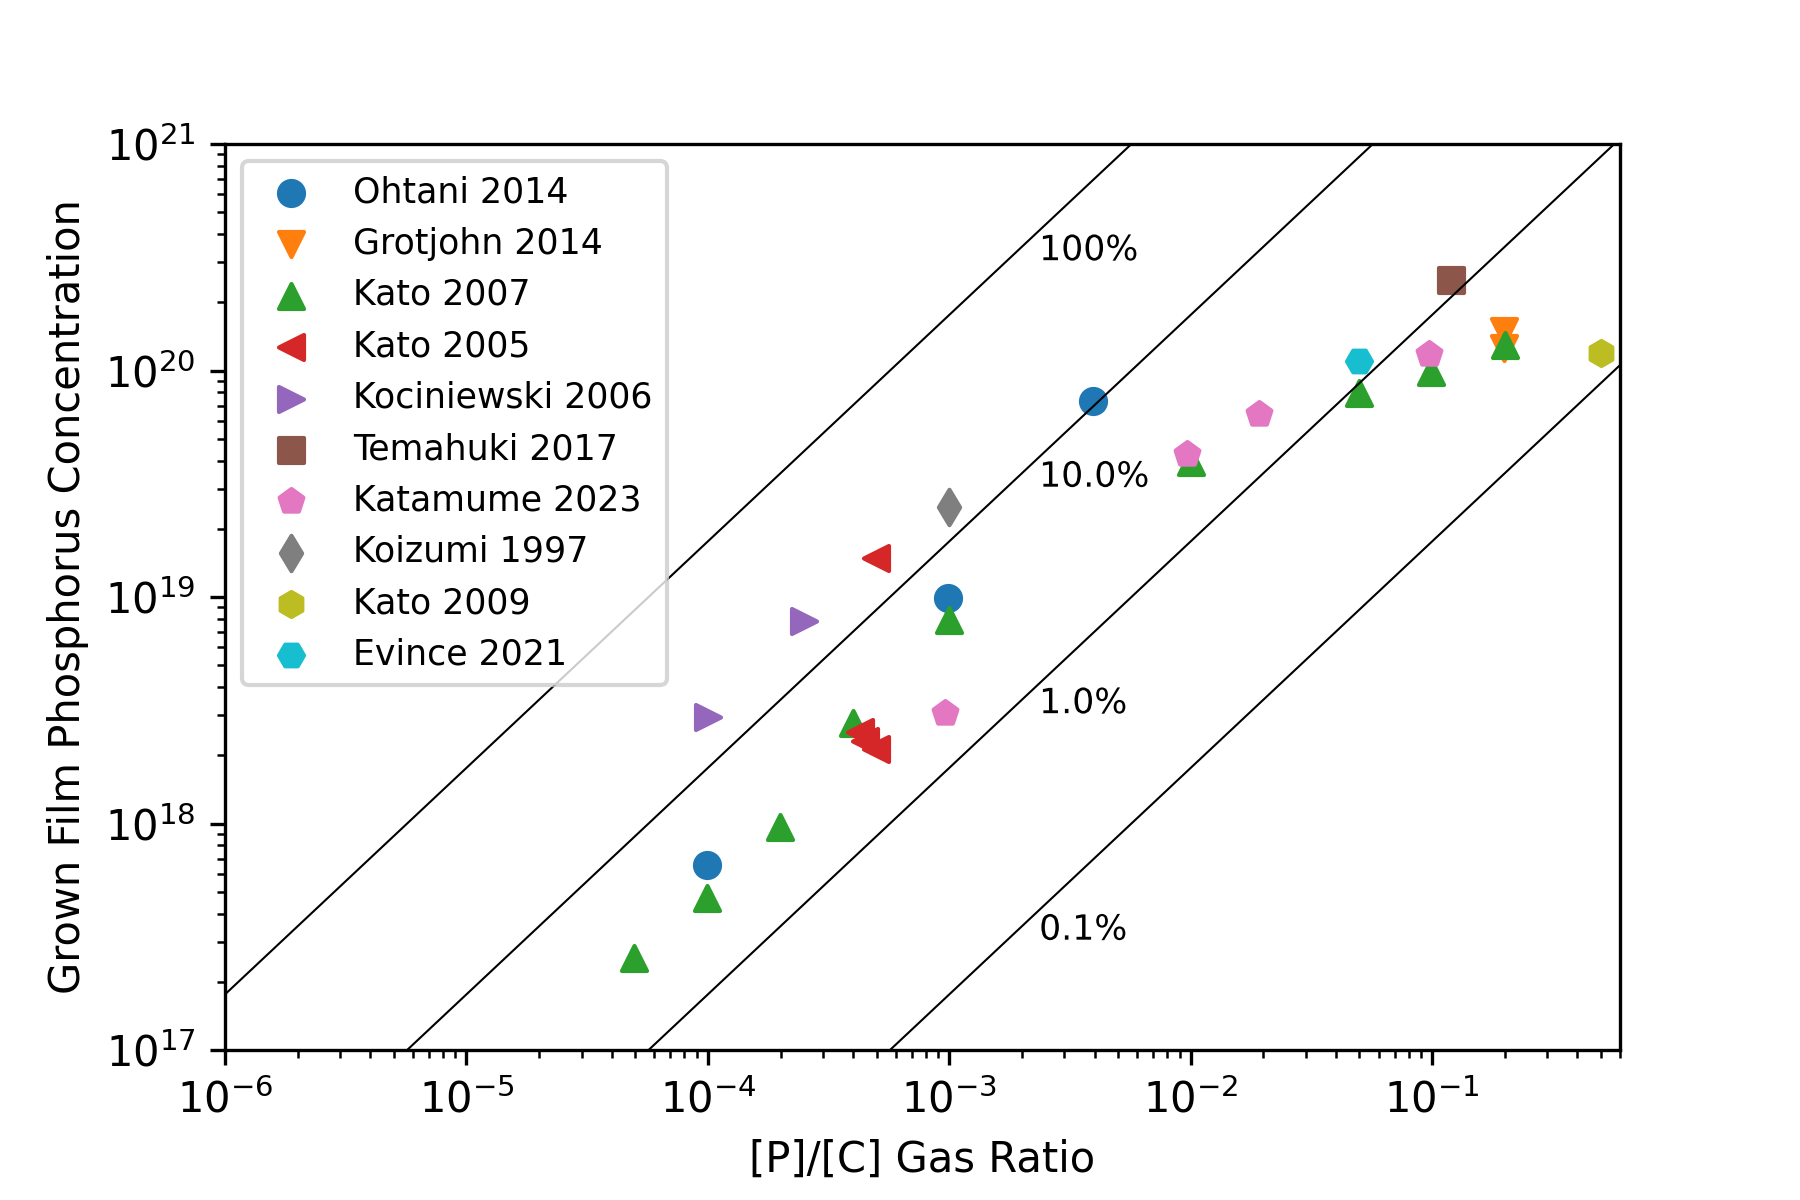
\includegraphics[width=\textwidth]{grown concentration vs gas ratio.png}
\caption{Phosphorus concentration of films as a function of measured [P]/[C] ratio. Each marker represents a different study, with scatter points indicating separate samples. The solid lines represent theoretical phosphorus concentrations for given efficiencies of phosphorus incorporation into the lattice.}
\label{fig:phos_concentration}
\end{figure}

\subsection{Phosphorous Incorporation}
Figure \ref{fig:phos_concentration} shows the efficiency of phosphorous incorporation from the gas phase into the resulting doped diamond lattice across various ratios. Theoretical efficiencies of incorporation, ranging from 100\% to 0.1\%, are represented as solid lines. The theoretical efficiency of incorporation for phosphorus from the gas phase into the resulting diamond lattice can be considered as:
\begin{equation}
\label{eq:incorporation_breakdown}
    \text{Incorporation efficiency} = \frac{\text{Resulting dopant concentration}}{\text{Dopant:carbon in CVD feedgas} \times \text{Atomic density of diamond}}
\end{equation}

For a detailed review of the different incorporation efficiencies as observed in the literature and how CVD growth has been optimised to improve this, please see section \ref{subsection:incorporation_efficiency}.

The phosphorous doped films as grown by Evince technology in 2021 and 2022 can be seen in the upper portion of P/C ratio growth, with both a relatively high ratio of 5\% phosphine in methane feedgas and a similarly high resultant diamond dopant concentration. This dopant concentration has been measured with SIMS in figures \ref{fig:sims_A}, \ref{fig:sims_B} and appears to match that of the literature comparisons.

\begin{figure}[h]
\centering
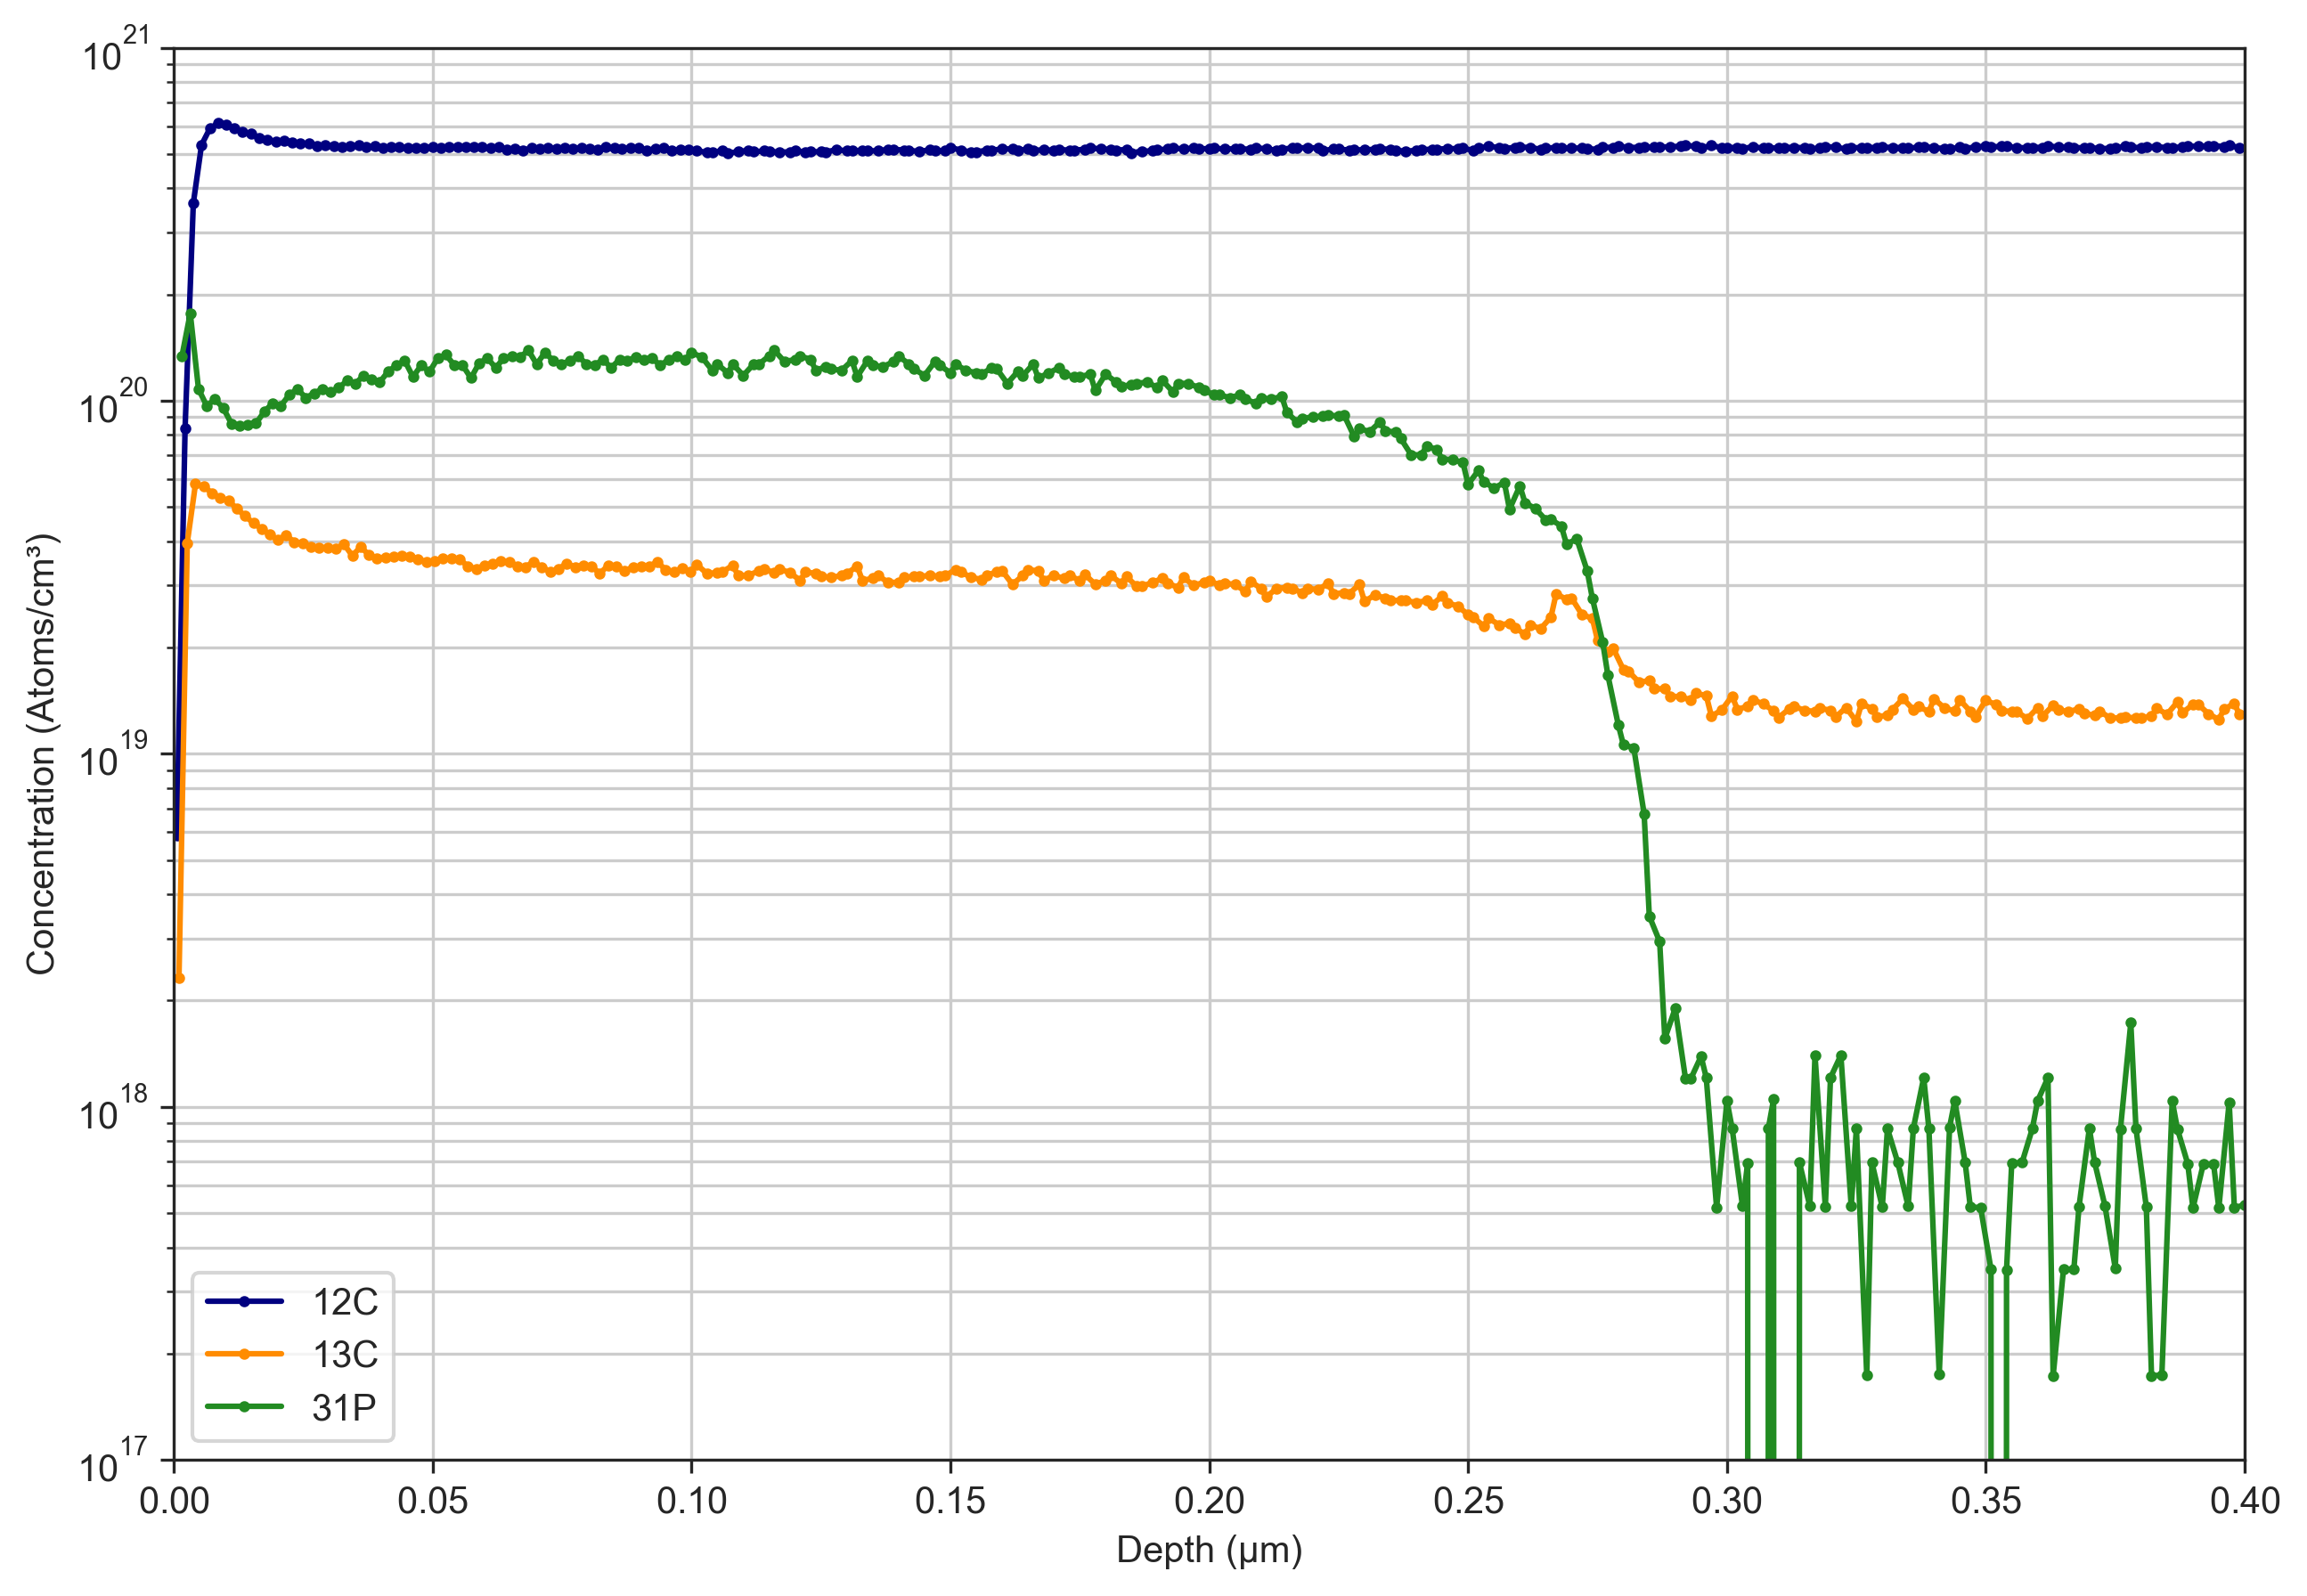
\includegraphics[width=\textwidth]{SIMS Depth Profile 49A.png}
\caption{The measured concentration of phosphorous in the grown film as measured via SIMS for sample A.}
\label{fig:sims_A}
\end{figure}

While figure \ref{fig:phos_concentration} does show a clear correlation of higher film concentrations with a higher ratio of phosphorous in the carbon containing gas phase, there is a limit at which this trend plateaus. The phosphorous concentration appears to reach saturation at around $10^{20}$ atoms/cm$^{3}$, which can be attributed to the limited solubility of phosphorous within the diamond lattice. For further discussion on the solubility of phosphorous within diamond, please see \ref{subsection:phosphorous_doping} in chapter 5. The phosphorous grown films from Evince appear to be at this saturation limit, with around $1\times10^{20}$ \si{\atoms\per\centi\metre\cubed} of phosphorous detected via SIMS to the $\approx1.76\times10^{23}$ \si{\atoms\per\centi\metre\cubed} of carbon within the diamond lattice.

The wide range of scatter points visible at specific P/C ratios suggests that factors beyond the P/C ratio, such as temperature, pressure, and plasma conditions (particularly in Microwave Plasma CVD growth), significantly influence the phosphorus concentration within grown films.

Furthermore, it suggests that the efficiency of phosphorus incorporation can vary between different growth techniques and experimental setups. The natural tendency for incorporation efficiency to diminish when higher concentrations of phosphorous are present in the gas phase could also be influenced by more than just solubility limitations. Factors such as changes in the plasma conditions, or the formation of phosphorous clusters which are not possible to incorporate into the diamond lattice, may also play a role.

\begin{figure}[h]
\centering
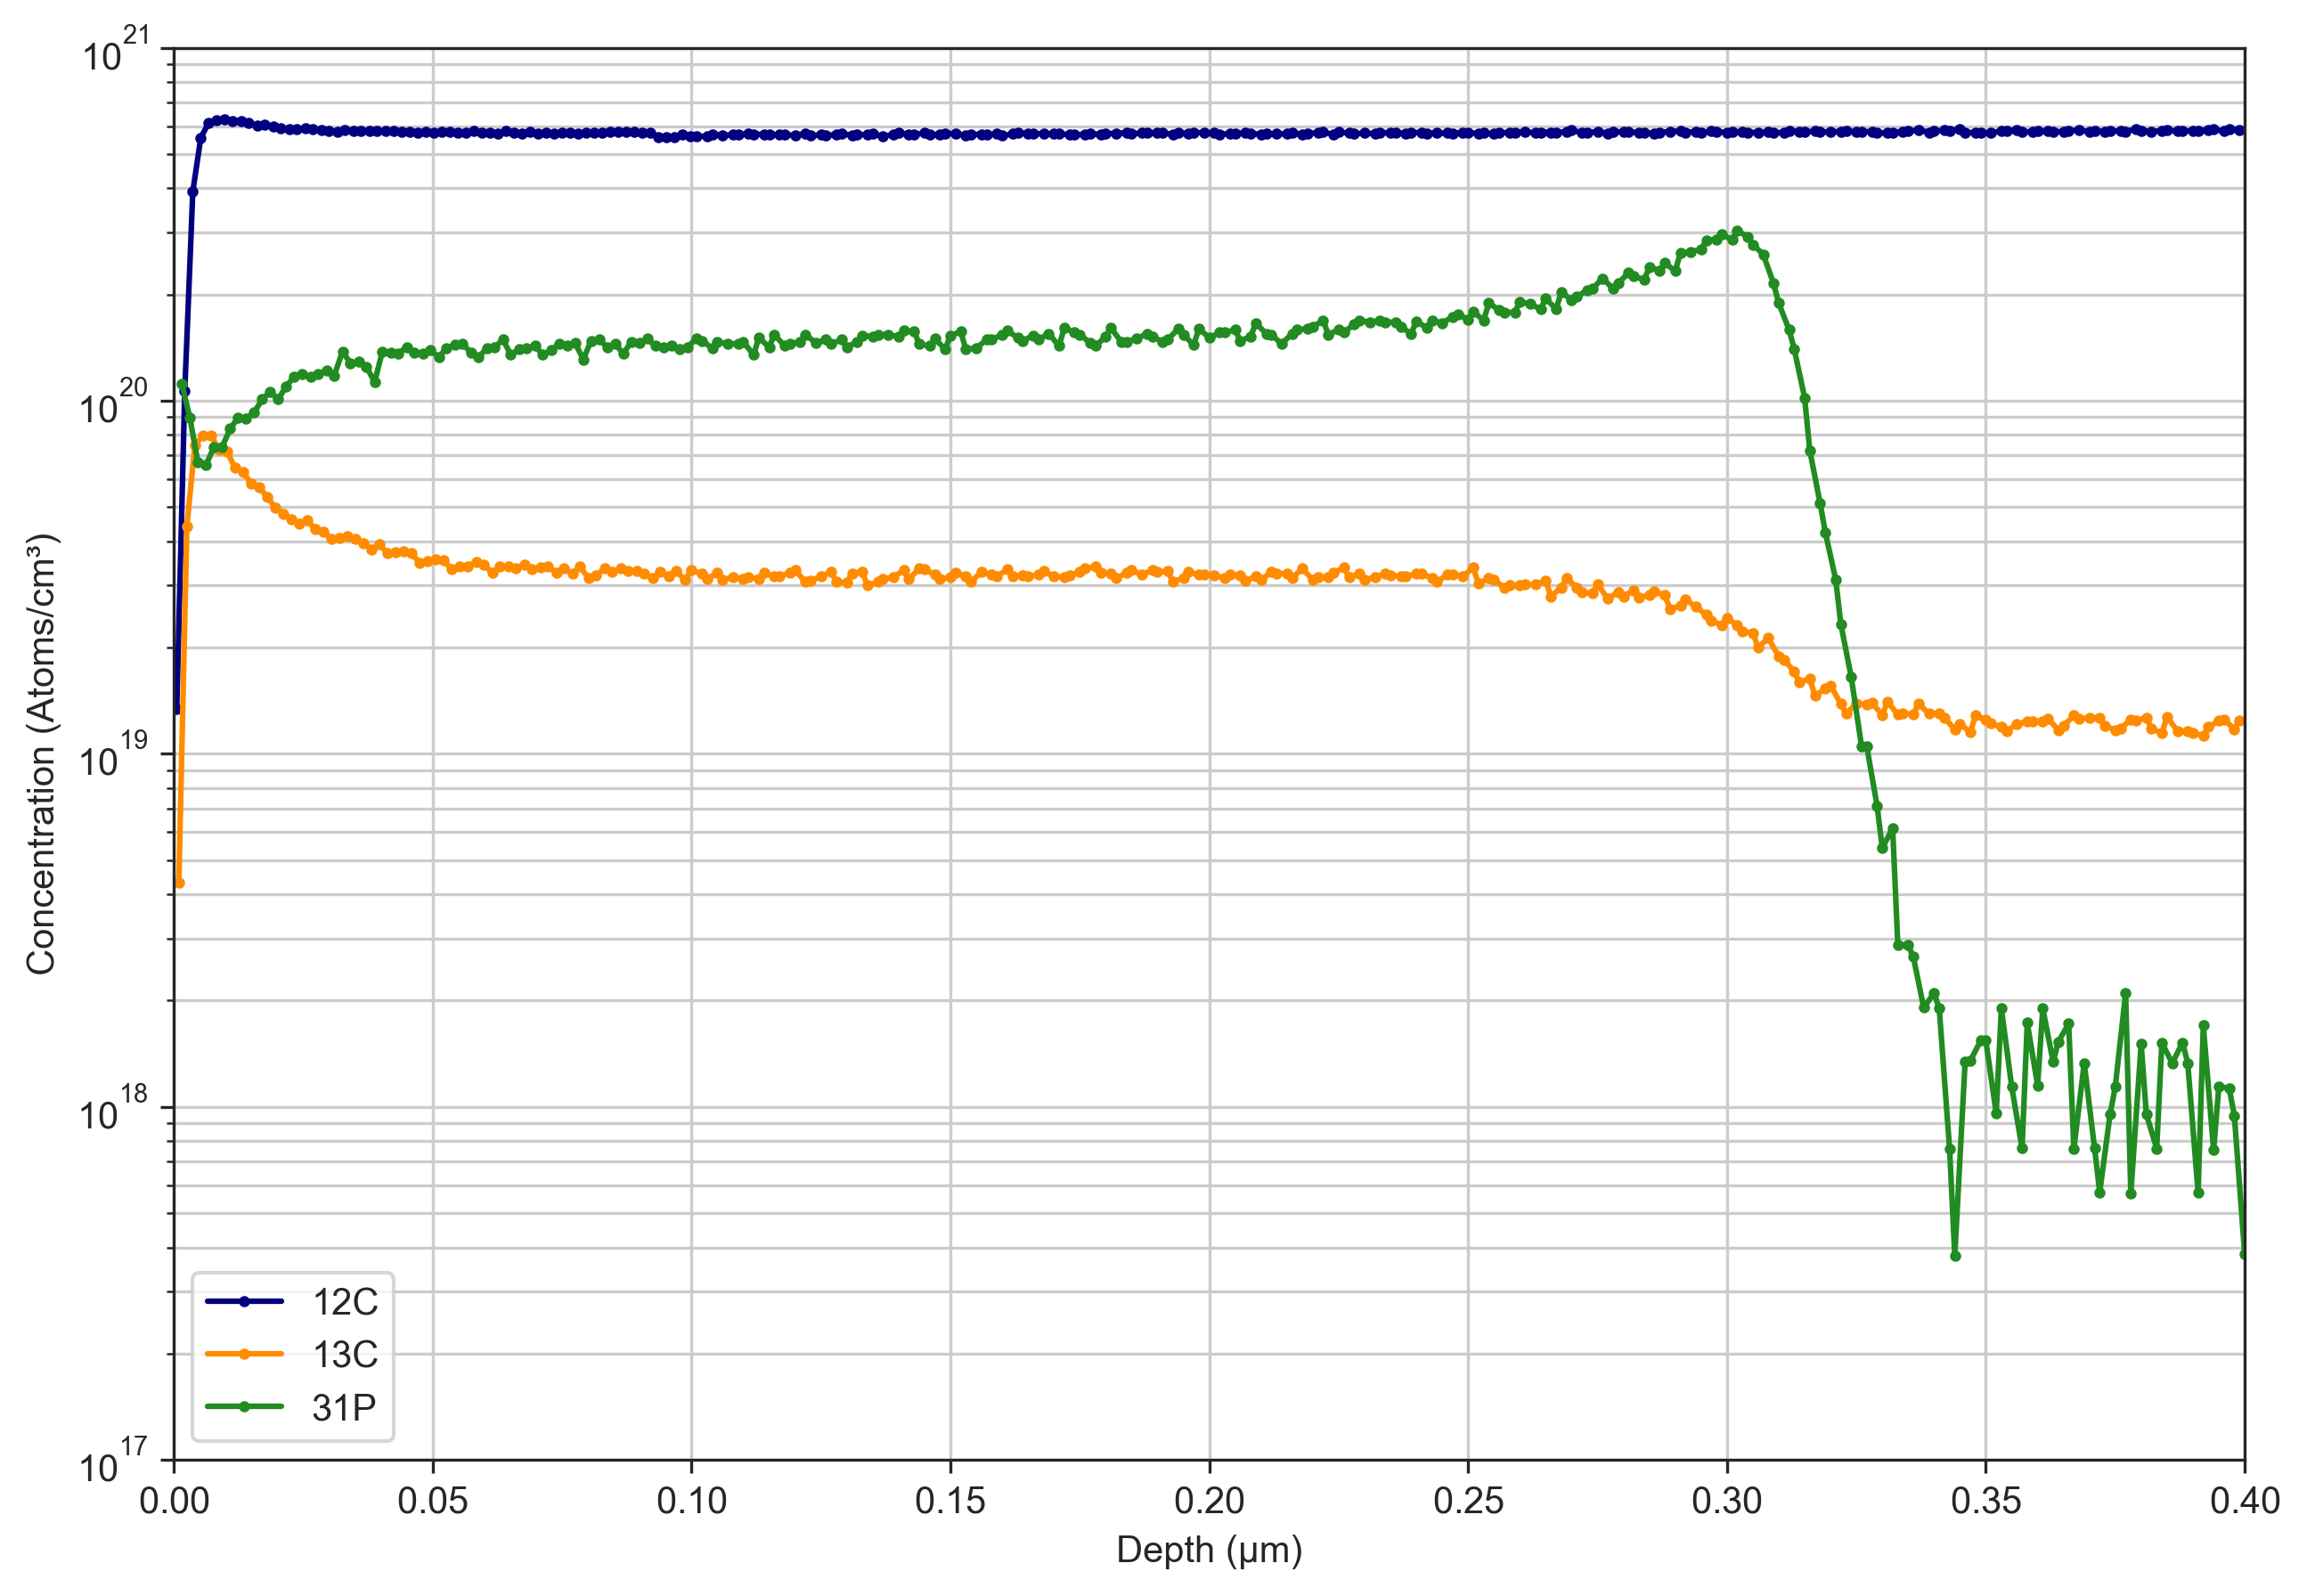
\includegraphics[width=\textwidth]{SIMS Depth Profile 63A.png}
\caption{The measured concentration of phosphorous in the grown film as measured via SIMS for sample B.}
\label{fig:sims_B}
\end{figure}
\subsubsection{SIMS Analysis}

SIMS analysis was performed on two samples to verify that the chosen growth conditions resulted in a highly doped phosphorous doped diamond film. This analysis was performed by Loughborough Surface Analysis Limited (LSA Ltd), with the results for samples A and B depicted in Figures \ref{fig:sims_A} and \ref{fig:sims_B}.

During SIMS analysis, LSA began monitoring with the minor carbon isotope, \ce{^{13}C}, and phosphorus. This choice allowed for a high instrument transmission, enabling the detection of low levels of phosphorus while maintaining the \ce{^{13}C} signal on the detector. Upon reaching the substrate, the \ce{^{13}C} signal noticeably decreased. This decrease prompted a shift to a lower instrument transmission and the additional monitoring of \ce{^{12}C}.

Throughout the profile, the \ce{^{12}C} signal remained consistent in both the layer and the substrate. By comparing the ratios of \ce{^{12}C} and \ce{^{13}C} to each other, it was observed that, while the ratio in the substrate aligned with the expected ratio for carbon, the \ce{^{13}C} signal was proportionally stronger in the epilayer. This discrepancy suggests a significant presence of hydrogen in the epilayer, which appears to combine with \ce{^{12}C}, resulting in an overall higher \ce{^{13}C} signal.

\subsection{Incomplete Ionisation}
At thermal equilibrium, the electron and hole contributions to current flow across a junction are equivalent, resulting in a constant Fermi level across such a junction. With this condition, the Poisson equation for anisotropic materials, determining the electrostatic potential $\psi$ can be simplified:

\begin{equation}
    \label{eq:poisson_3.10_tesfaye}
\end{equation}
\begin{equation}
    n + N^{-}_{a}=p+N^{+}_{d}
    \label{eq:poisson_simplified_tesfaye}
\end{equation}

Then solved with the mass action law:

\begin{equation}
    n\cdot p = n^{2}_{i}
    \label{eq:intrinsic_carriers_3.69_tesfaye}
\end{equation}

To give the equilibrium electron or hole concentration in an n or p-type material respectively:

\begin{equation}
    n=\frac{1}{2}\cdot\left(N^{+}_{d}-N^{-}_{a}+\sqrt{\left(N^{+}_{d}-N^{-}_{a}\right)^{2}-4n^{2}_{i}}\right)
    \label{eq:equilibrium_electron_concentration_3.121_tesfaye}
\end{equation}
\begin{equation}
    p=\frac{1}{2}\cdot\left(N^{-}_{a}-N^{+}_{d}+\sqrt{\left(N^{+}_{d}-N^{-}_{a}\right)^{2}-4n^{2}_{i}}\right)
\end{equation}

The concentration of ionised impurity atoms is then given by a steady-state Gibbs distribution as in \cite{tcadmanual2001}:
\begin{equation}
    N^{+}_{d} = \frac{N_{d}}{1+g_{d}\cdot\frac{n}{n_{1}}}
    \label{eq:incomplete_ionisation_donors}
\end{equation}
With: 
\begin{equation}
    n_{1}=N_{c}\cdot\exp{-\frac{E_{c}-E_{d}}{k\cdot T}}
    \label{eq:n_{1}_gibbs_distribution}
\end{equation}
Or:
\begin{equation}
    N^{+}_{a} = \frac{N_{a}}{1+g_{a}\cdot\frac{p}{p_{1}}}
    \label{eq:incomplete_ionisation_acceptors}
\end{equation}
With:
\begin{equation}
    p_{1}=N_{v}\cdot\exp{-\frac{E_{a}-E_{v}}{k\cdot T}}
    \label{eq:p_{1}_gibbs_distribution}
\end{equation}

Where $N_{d,a}$ are the substitutional and hence active dopant concentrations of donors and acceptors respectively. The ground state degeneracy factor for the donor impurity level in diamond $g_{d} = 2$, since a donor level can accept one electron with either spin, or have no electron at all  (\cite{koizumi2018:ch2}. The ground state degeneracy factor for acceptor levels is $g_{a}=4$ as each acceptor impurity level can accept a hole of either spin, with a doubly degenerate impurity level as a result of the two degenerate valence bands at $\Vec{k}=0$.

It can also be more convenient to express the ionisation fraction in terms of the carrier concentrations, instead of the relevant quasi-Fermi levels. Taking the Fermi-Dirac statistics form of the carrier concentrations, rather than the Maxwell-Boltzmann form, simply adds the $\gamma_{n,p}$ parameter:

\begin{equation}
    n_{2}=N_{c}\gamma_{n}\cdot\exp{-\frac{E_{c}-E_{f}}{k\cdot T}}
    \label{eq:n_{2}_fermi_distribution}
\end{equation}

\begin{equation}
    p_{2}=N_{c}\gamma_{p}\cdot\exp{-\frac{E_{fp}-E_{v}}{k\cdot T}}
    \label{eq:p_{2}__fermi_distribution}
\end{equation}

In the non-degenerate limit, the Fermi-Dirac distribution gives the Maxwell-Boltzmann distribution and $\gamma_{n,p}=1$. This can be used to define the relevant quasi-Fermi levels as:

\begin{equation}
    E_{fn} = kT\ln{\frac{n}{\gamma_{n}N_{c}}}+E_{c}
    \label{eq:quasi-fermi_levels_carriers_n}
\end{equation}

\begin{equation}
    E_{fp} = -kT\ln{\frac{n}{\gamma_{p}N_{v}}}+E_{v}
    \label{eq:quasi-fermi_levels_carriers_p}
\end{equation}

With the resulting fraction of ionised carriers given in the form:

\begin{equation}
    \frac{N_{d}^{+}}{N_{d}} = \frac{1}{1+\frac{g_{d}n}{\gamma_{n}N_{c}}\exp{\frac{\Delta E_{d}}{kT}}}
    \label{eq:incomplete_ionisation_final_n}
\end{equation}

\begin{equation}
    \frac{N_{a}^{+}}{N_{a}} = \frac{1}{1+\frac{g_{a}p}{\gamma_{p}N_{v}}\exp{\frac{\Delta E_{a}}{kT}}}
    \label{eq:incomplete_ionisation_final_p}
\end{equation}

\begin{figure}[h]
    \centering
    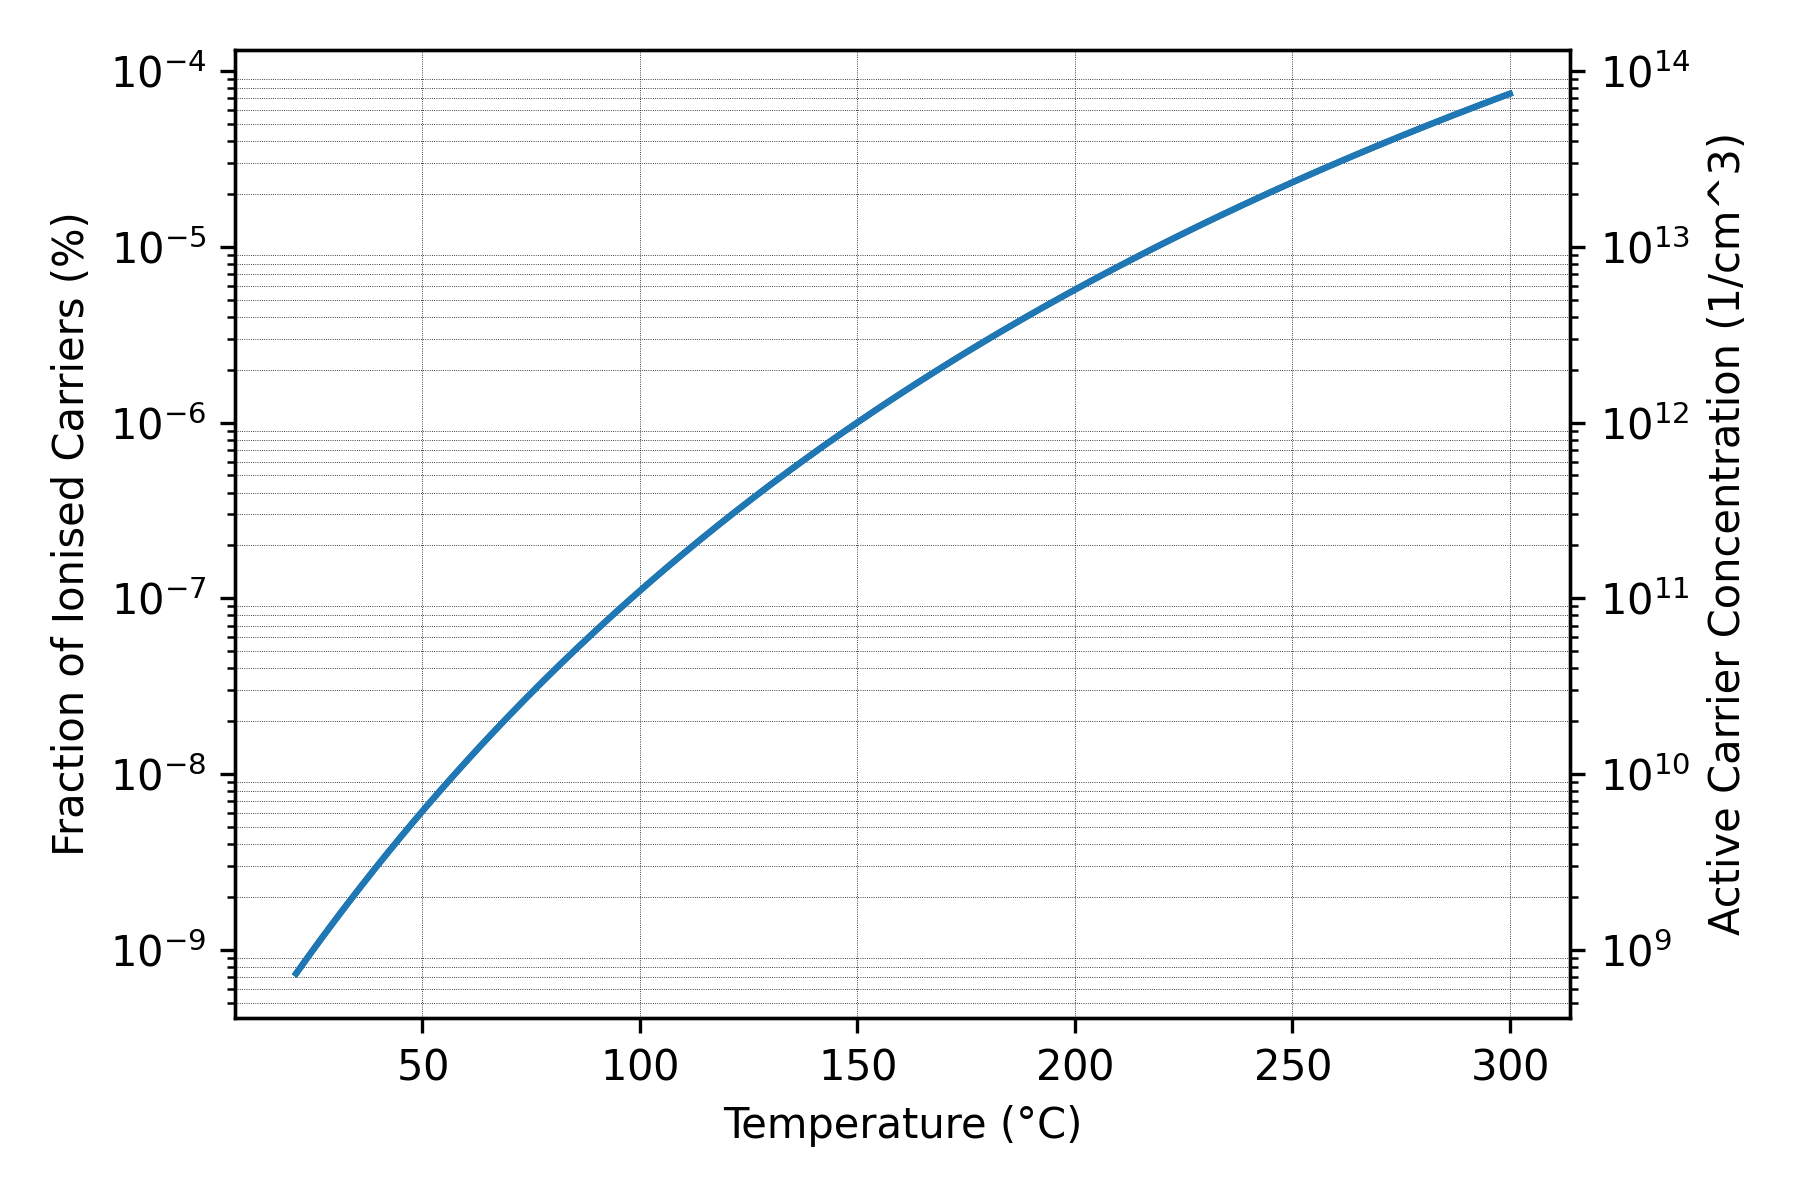
\includegraphics[width=0.97\textwidth]{active_carriers.png}
    \caption{The number of active carriers according to the thermal ionisation equation with a donor energy level of 0.6 \si{\electronvolt}}
    \label{fig:active_carriers}
\end{figure}

Where $\Delta E_{d}=E_{c}-E_{d}$ and $\Delta E_{a}=E_{a}-E_{v}$. The results of this equation for phosphorous are shown in figure \ref{fig:active_carriers}. At room temperature with a phosphorous concentration of $1\times10^{20}$ \si{\per\centi\metre\cubed}, the active carrier concentration can be as low as $5.25\times10^{9}$ \si{\per\centi\metre\cubed}, or $5.25\times10^{-9}\%$ which is also demonstrated in other works with hall effect measurements. At 300\si{\degreeCelsius} this is raised to an active carrier concentration of $5.30\times10^{14}$ \si{\per\centi\metre\cubed}, or $5.30\times10^{-4}\%$ of the doping concentration. Hence, this will be a significant factor in the sheet resistance of phosphorous doped diamond. 


\subsubsection{Partly compensated donors}
Along with the thermal ionisation of donors, it is also important to consider the compensation of donors within diamond. The effective carrier concentration, taking into account the presence of compensating acceptor states, can be given with the following equation:
\begin{equation}
    \frac{n\left(N_{A}+n\right)}{N_{D}-N_{A}-n} = \frac{N_{C}}{g_{d}}\exp{-\frac{E_{d}}{kT}}
    \label{eq:carrier_compensation_koizumi2018}
\end{equation}
Where the activation energy $E_{d}=E_{c}-E_{d}$, the degeneration factor $g_{d} = 2$, $N_{D,A}$ are the carrier concentrations, $k$ is the Boltzmann constant, $T$ is the temperature and $N_{C}$ is the effective density of state, expressed in this case as:
\begin{equation}
    N_{C} = 12\left(\frac{2\pi m^{*}_{e}kT}{h^{2}}\right)^{3/2}
    \label{eq:carrier_compensation_density_of_state}
\end{equation}
Where the effective mass of donor electrons $m^{*} = 0.55m_{e}$ ($m_{e}$) is the mass of a free electron) and $h$ is the Plank constant. Previous work has 
\subsection{Ti/Pt/Au Contacts}
\begin{table}[h]
\centering
\caption{A trimmed copy of table \ref{table:samples_summary}, including relevant samples for this subsection.}
\label{table:short_samples_summary}
\begin{tabular}{|c|c|c|c|c|}
\hline
Sample & Batch & Thickness (\si{\micro\metre}) & Contacts & Characterisation \\
\hline
A & 1 & 0.3 & None & SIMS \\
B & 1 & 0.3 & None & SIMS \\
C & 2 & 0.3 & Ti/Pt/Au - 850\si{\degreeCelsius} 30 mins  & TLM, AFM \\
D & 2 & 0.3 & Ti/Pt/Au - 600\si{\degreeCelsius} 300 mins & TLM, AFM \\
% Add more samples here
\hline
\end{tabular}
\end{table}
Two samples (C and D) were used for initial TLM characterisation. With the same growth conditions as for samples A and B, a heavily phosphorous doped surface layer was grown via MPCVD following the standard cleaning process. In figure \ref{fig:TLMB} the final Ti/Pt/Au structure used for both is shown. The linear TLM structure can be seen on the lower portion of the sample's surface. When compared, the sample dimensions were comparable, with sizes of $3.7\times3.8$ \si{\milli\metre} for sample C and $3.9\times4.1$ \si{\milli\metre} for sample D. The Ti/Pt/Au contacts used were fabricated via electron-beam lithography, with thicknesses of 20/20/100 \si{\micro\metre} respectively. Sample C was annealed at 850\si{\degreeCelsius} for 30 minutes, while sample D was annealed at 600\si{\degreeCelsius} for 300 minutes, as summarised in table \ref{table:short_samples_summary}. Annealing conditions were chosen such that a shorter, 'high' temperature anneal could be compared to a longer, 'low' temperature anneal. Crucial to the success of such annealing is the formation of TiC at the diamond interface, which is examined further in section \ref{subsubsec:annealing}, but generally is observed from temperatures as low as $400$ \si{\degreeCelsius}.

The surface thicknesses for samples C and D are estimated at 0.3 \si{\micro\metre}, as while grown in different batches, the duration of phosphorous growth was consistent between batch 1 and 2, hence the SIMS data for samples A and B may be considered representative for these subsequent samples.

\begin{figure}[h]
\centering
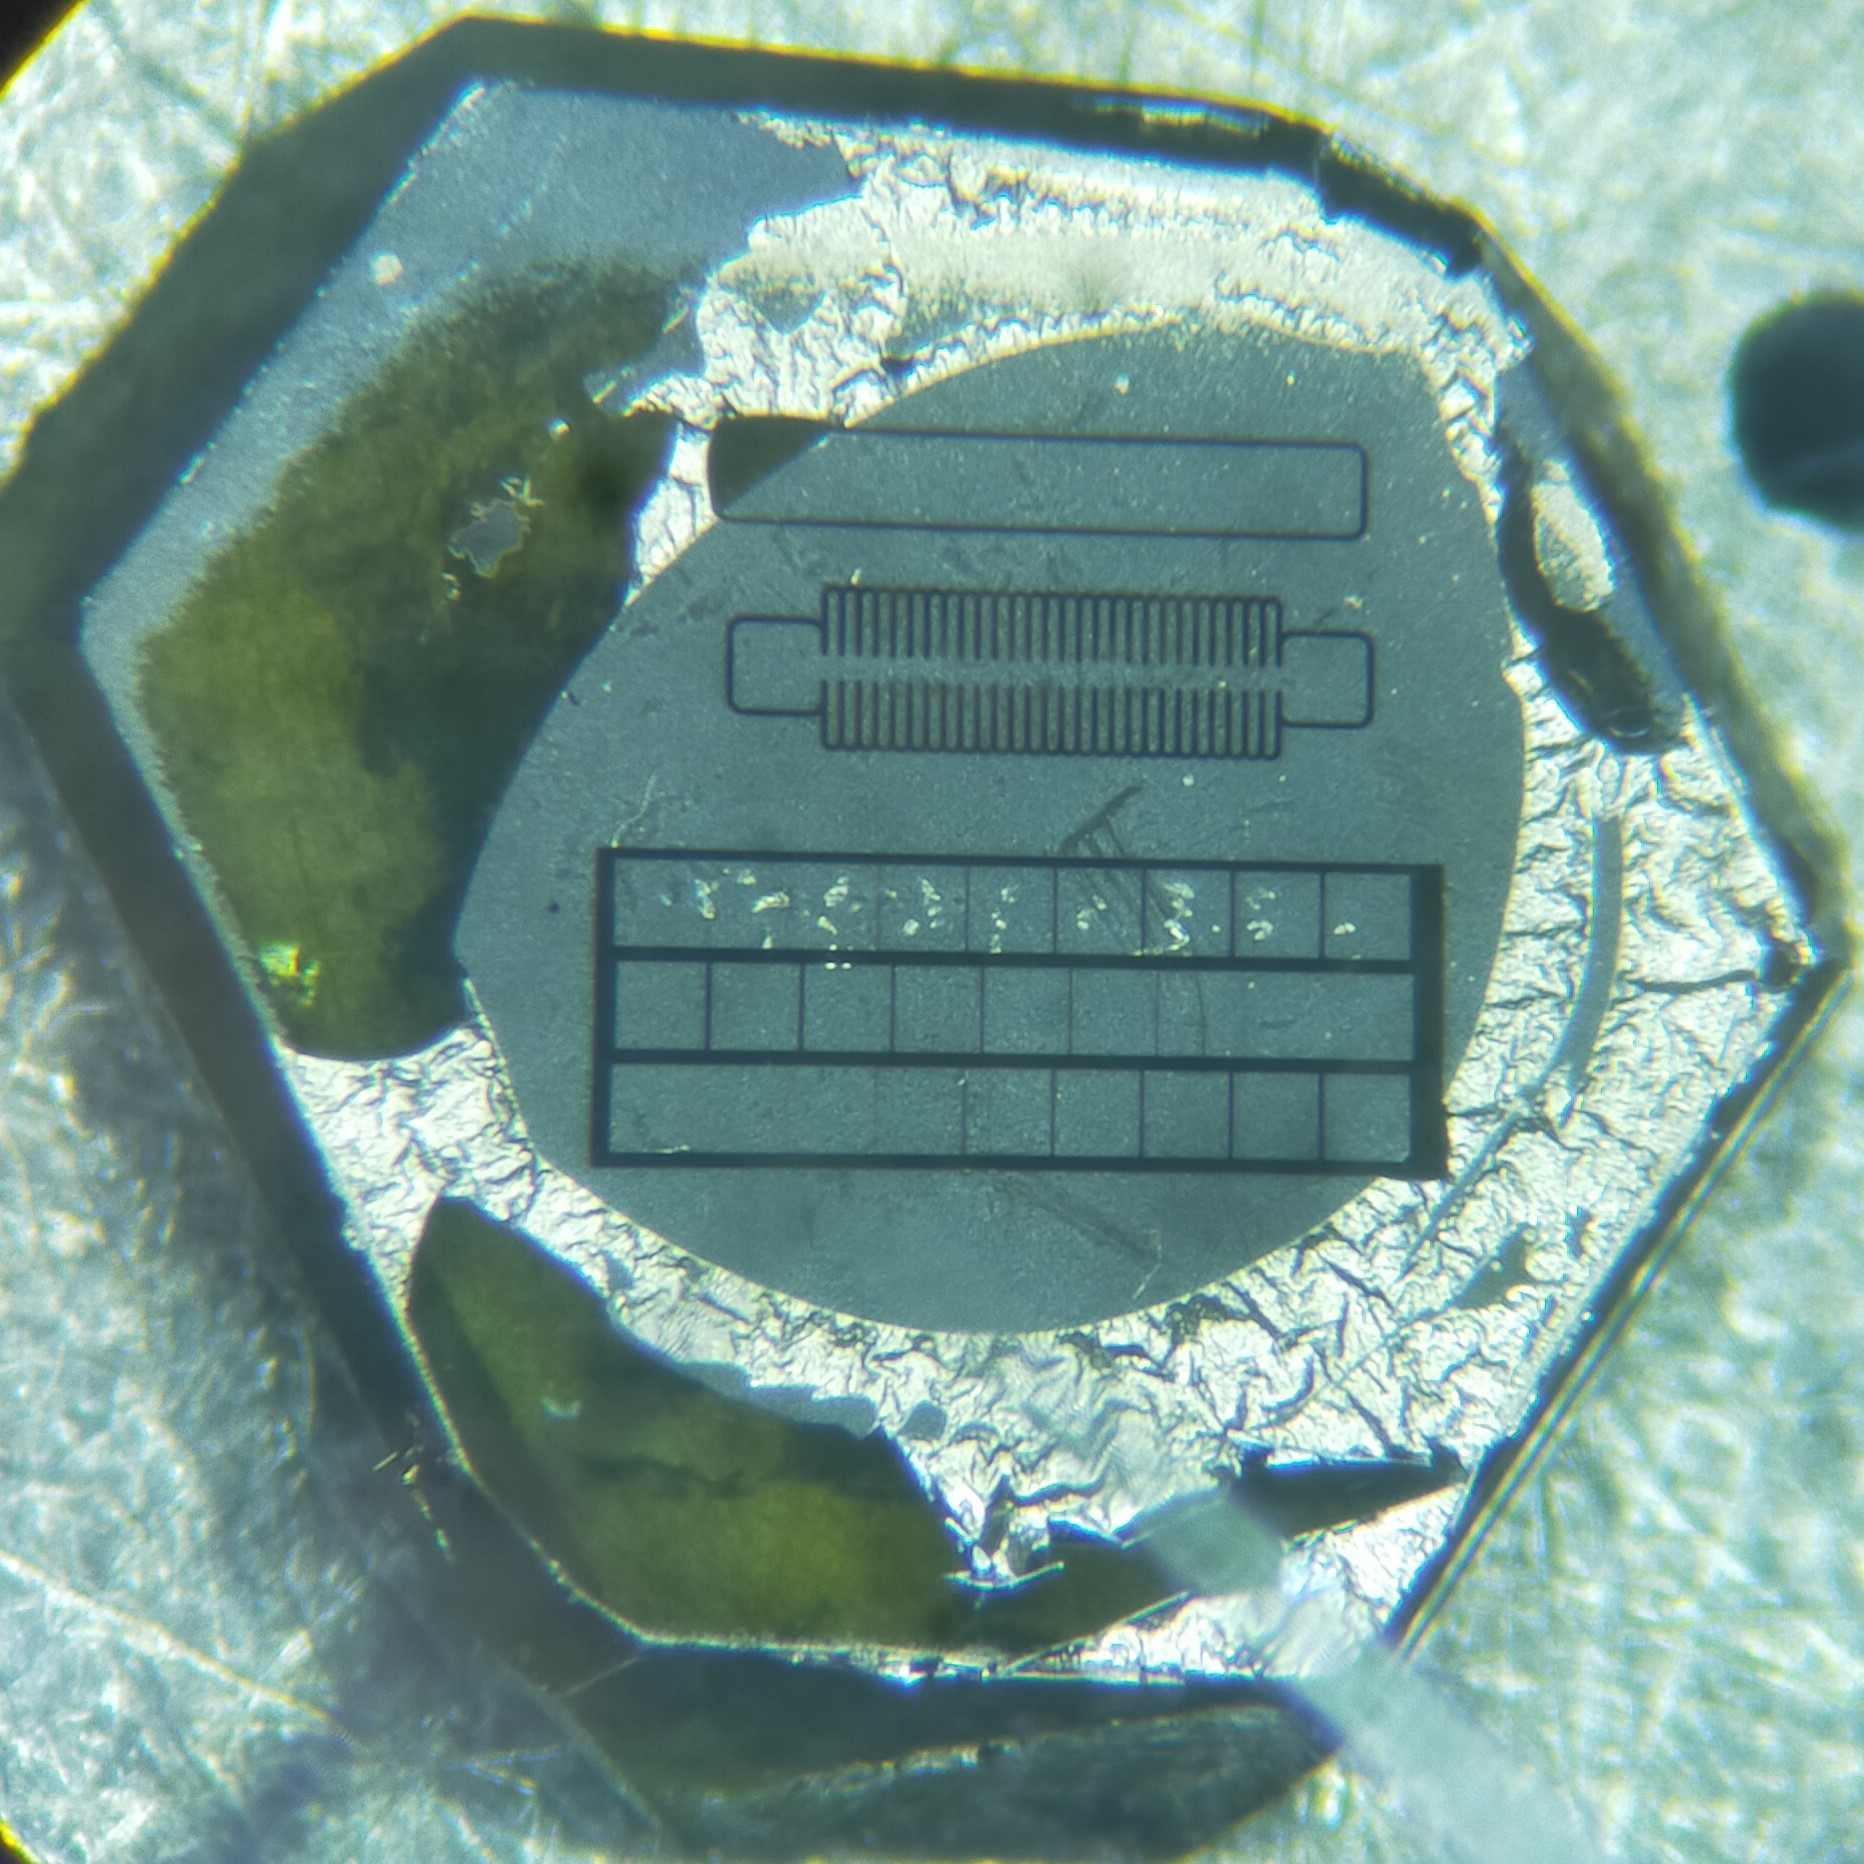
\includegraphics[width=0.6\textwidth]{Chapter6/Figs/Raster/Sample D 2019/TLMB.jpg}
\caption{Sample B with linear TLM contacts, as seen with an optical microscope.}
\label{fig:TLMB}
\end{figure}

\section{Linear Transfer Length Method (TLM)}
In this section, the measured I-V curves for samples C and D ranging from room temperature to 300\si{\degreeCelsius} are analysed. Due to the phosphorous donor ionisation energy of around 0.6 \si{\electronvolt}, there is a very significant temperature dependence. At room temperature, the smallest channel width of approximately 3.5 \si{\micro\metre} drew a current of approximately $1.57\times10^{-6}$\si{\ampere\per\centi\metre\squared} with a potential bias of 10 \si{\volt}, while at 300\si{\degreeCelsius} this increased to $1.08\times10^{-4}$\si{\ampere\per\centi\metre\squared}. 

\subsection{Ti/Pt/Au I-V Results}
The linear plots of measured current vs applied voltage for samples C and D for temperatures of 21, 150 and 300 \si{\degreeCelsius} are presented in this section, for a bias range of $\pm10$ \si{\volt}. For a full set of I-V data please see section \ref{app:LTLM_I_V_data}.

For reference, error bars of 2 \si{\pico\ampere} are plotted on a limited bias range of $\pm1$ \si{\volt} in figure \ref{fig:1V_C_current_voltage_21} to examine the potential magnitudes of error. Typical errors for the B1500A as calibrated are typically no higher than 1 \si{\pico\ampere} as calibrated, with the measured data hence only showing noise when the applied bias is close to 0 \si{\volt}.

\begin{figure}[h]
    \centering
    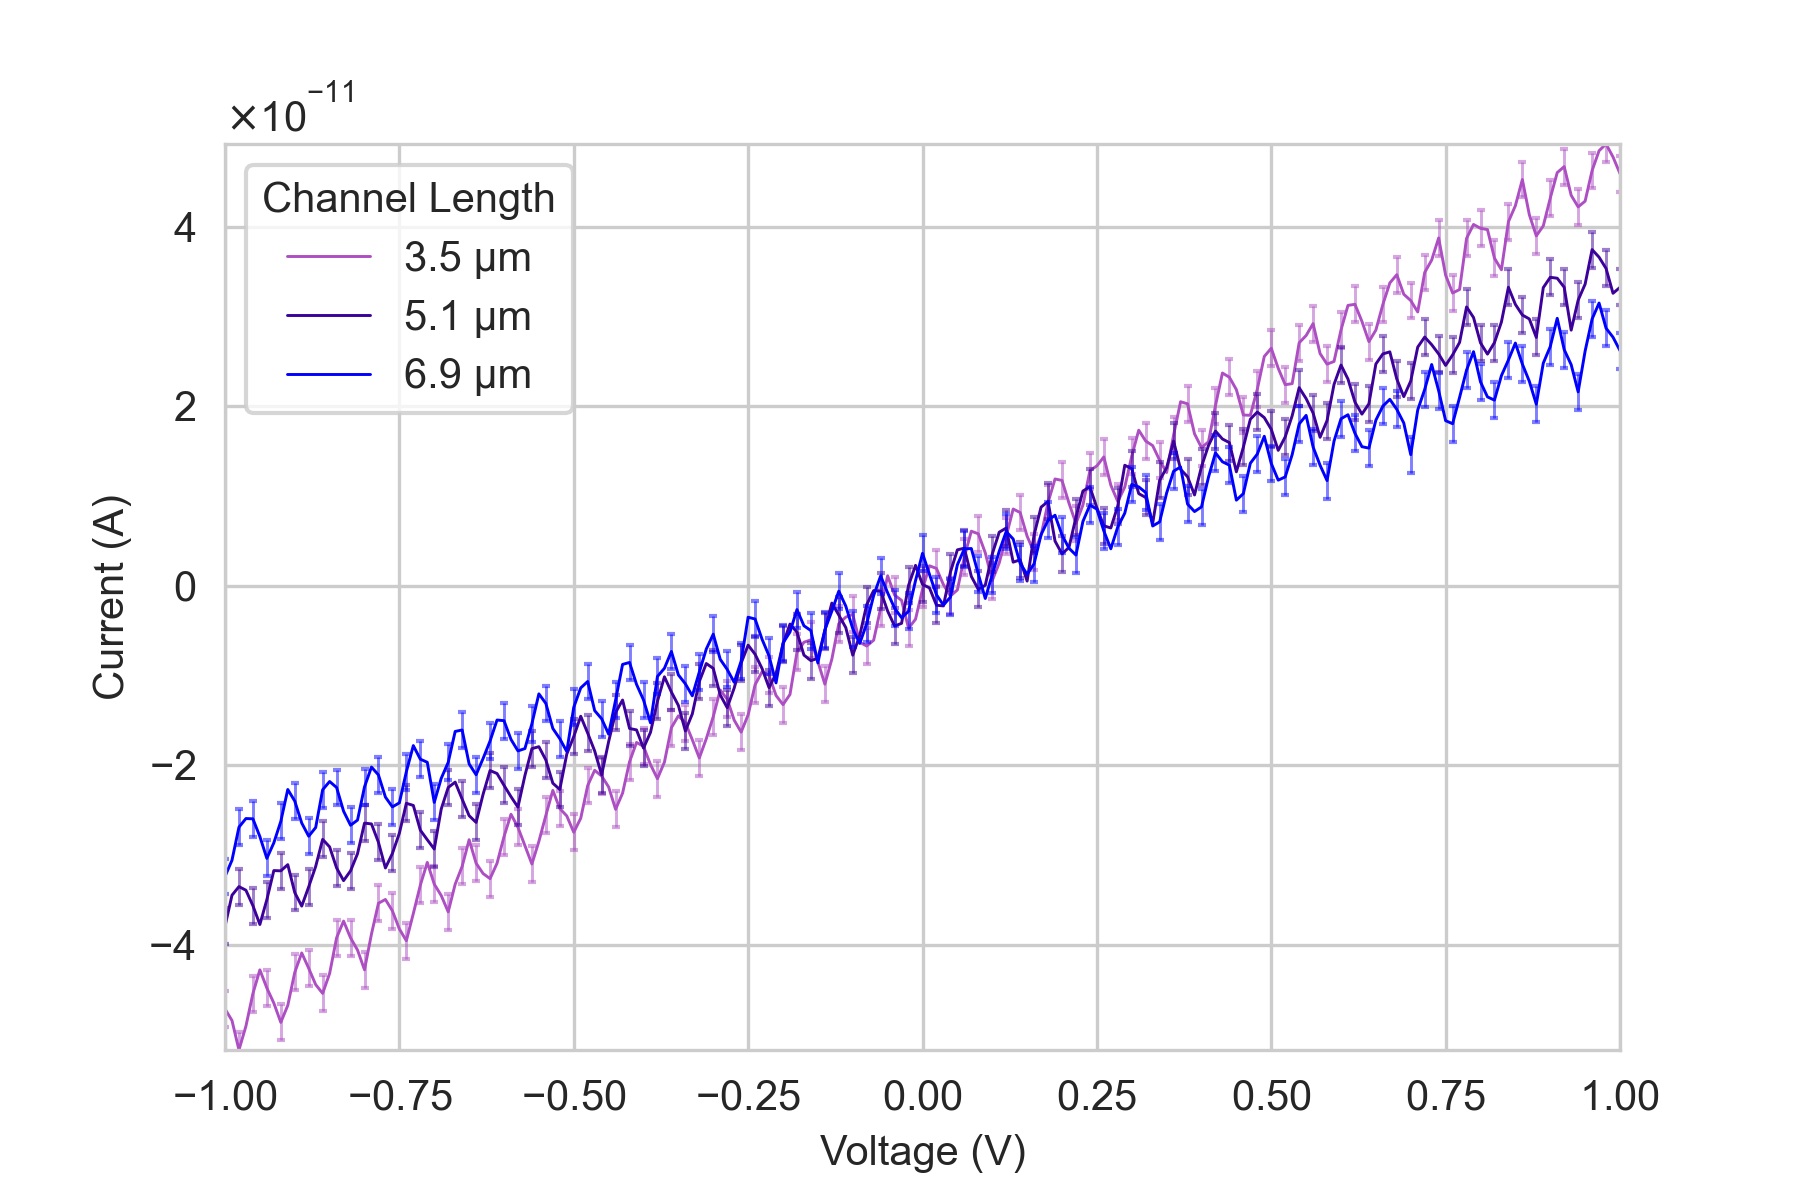
\includegraphics[width=0.97\textwidth]{Appendix1/1V IV characteristics at 21 C.png}
    \caption{A linear plot of the measured current against applied voltage for three channel lengths, $\pm1$ \si{\volt}, with 2 \si{\pico\ampere} error bars at 21\si{\degreeCelsius} (sample C).}
    \label{fig:1V_C_current_voltage_21}
\end{figure}

\begin{figure}[h]
    \centering
    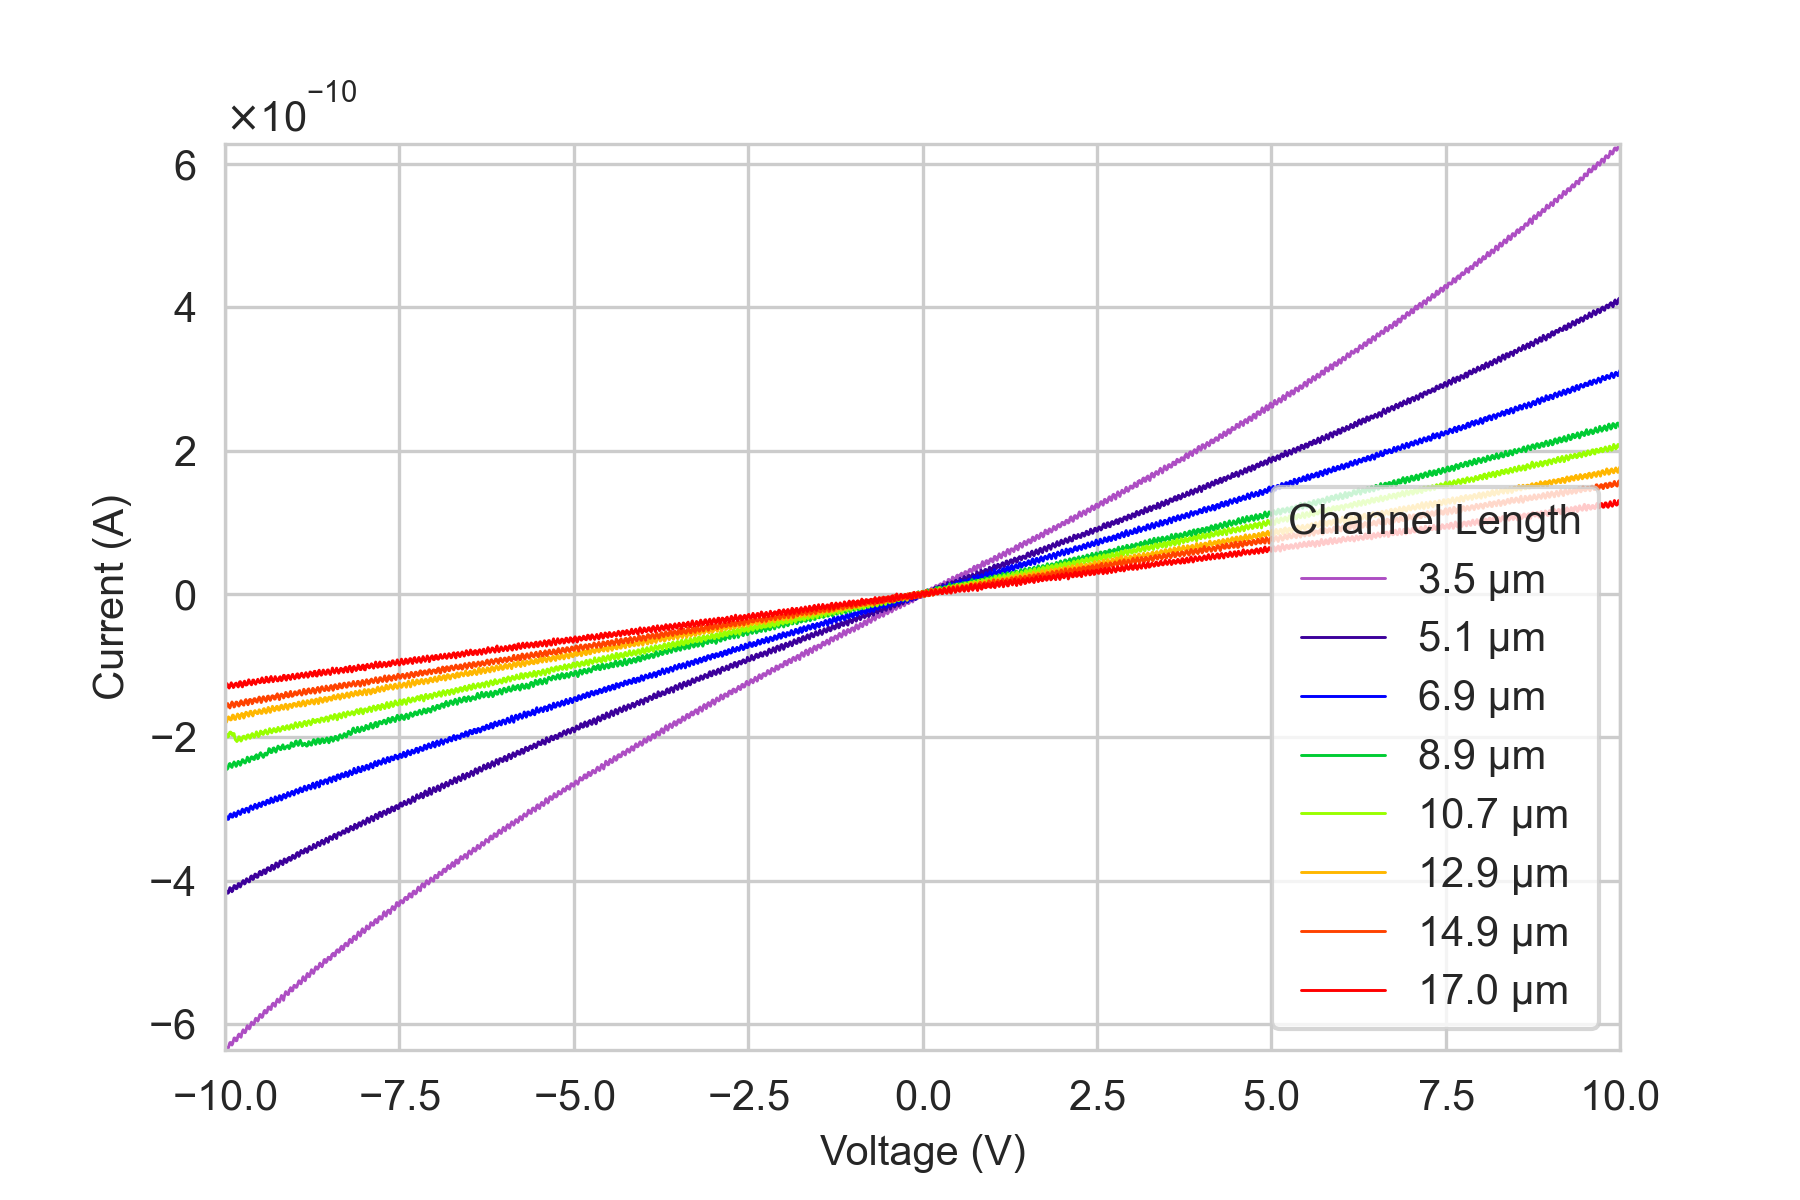
\includegraphics[width=0.97\textwidth]{Chapter6/Figs/Raster/Sample C 2019/IV/10V IV characteristics at 21 C.png}
    \caption{A linear plot of the measured current against applied voltage for all channel lengths at 21\si{\degreeCelsius} (sample C).}
    \label{fig:C_current_voltage_21}
\end{figure}
\begin{figure}[h]
    \centering
    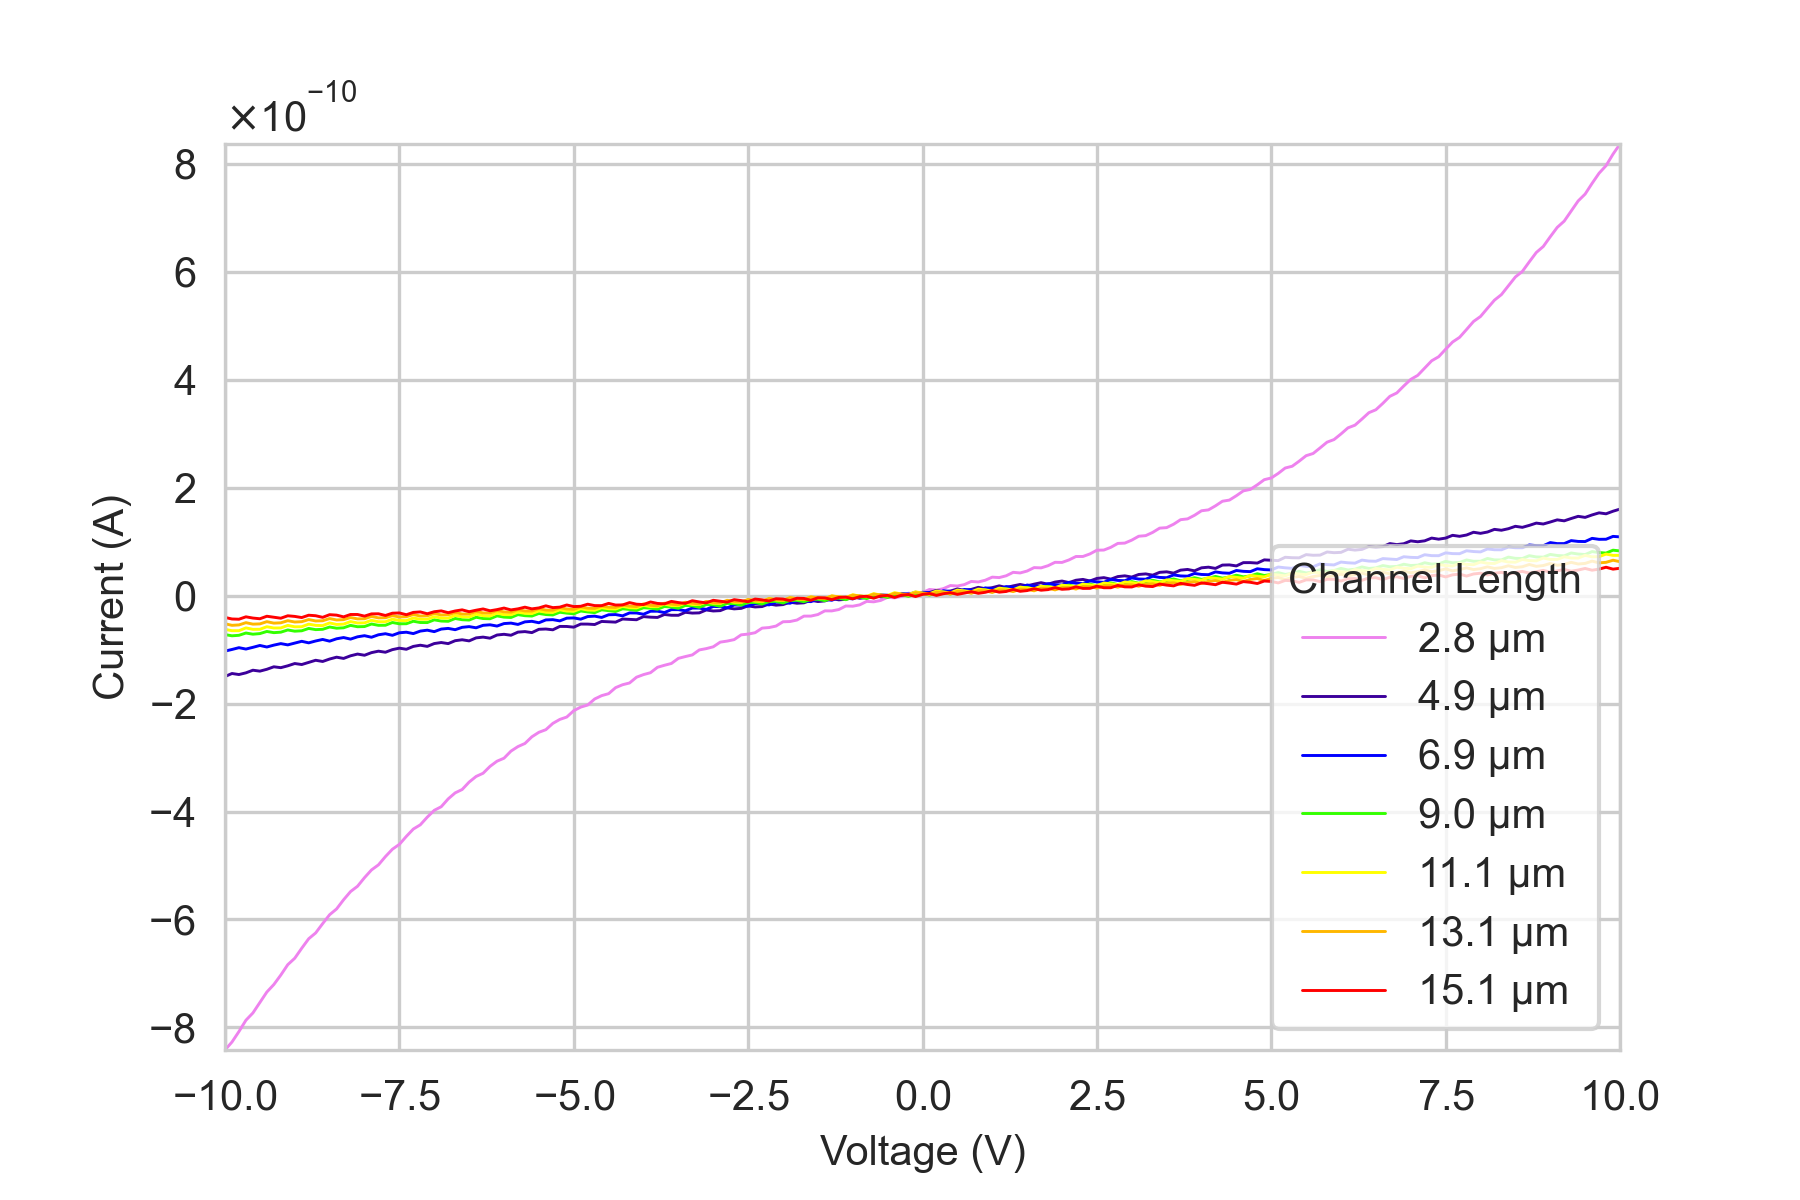
\includegraphics[width=0.97\textwidth]{Chapter6/Figs/Raster/Sample D 2019/IV/10V IV characteristics at 21 C.png}
    \caption{A linear plot of the measured current against applied voltage for all channel lengths at 21\si{\degreeCelsius} (sample D).}
    \label{fig:D_current_voltage_21_10V}
\end{figure}

\begin{figure}[h]
    \centering
    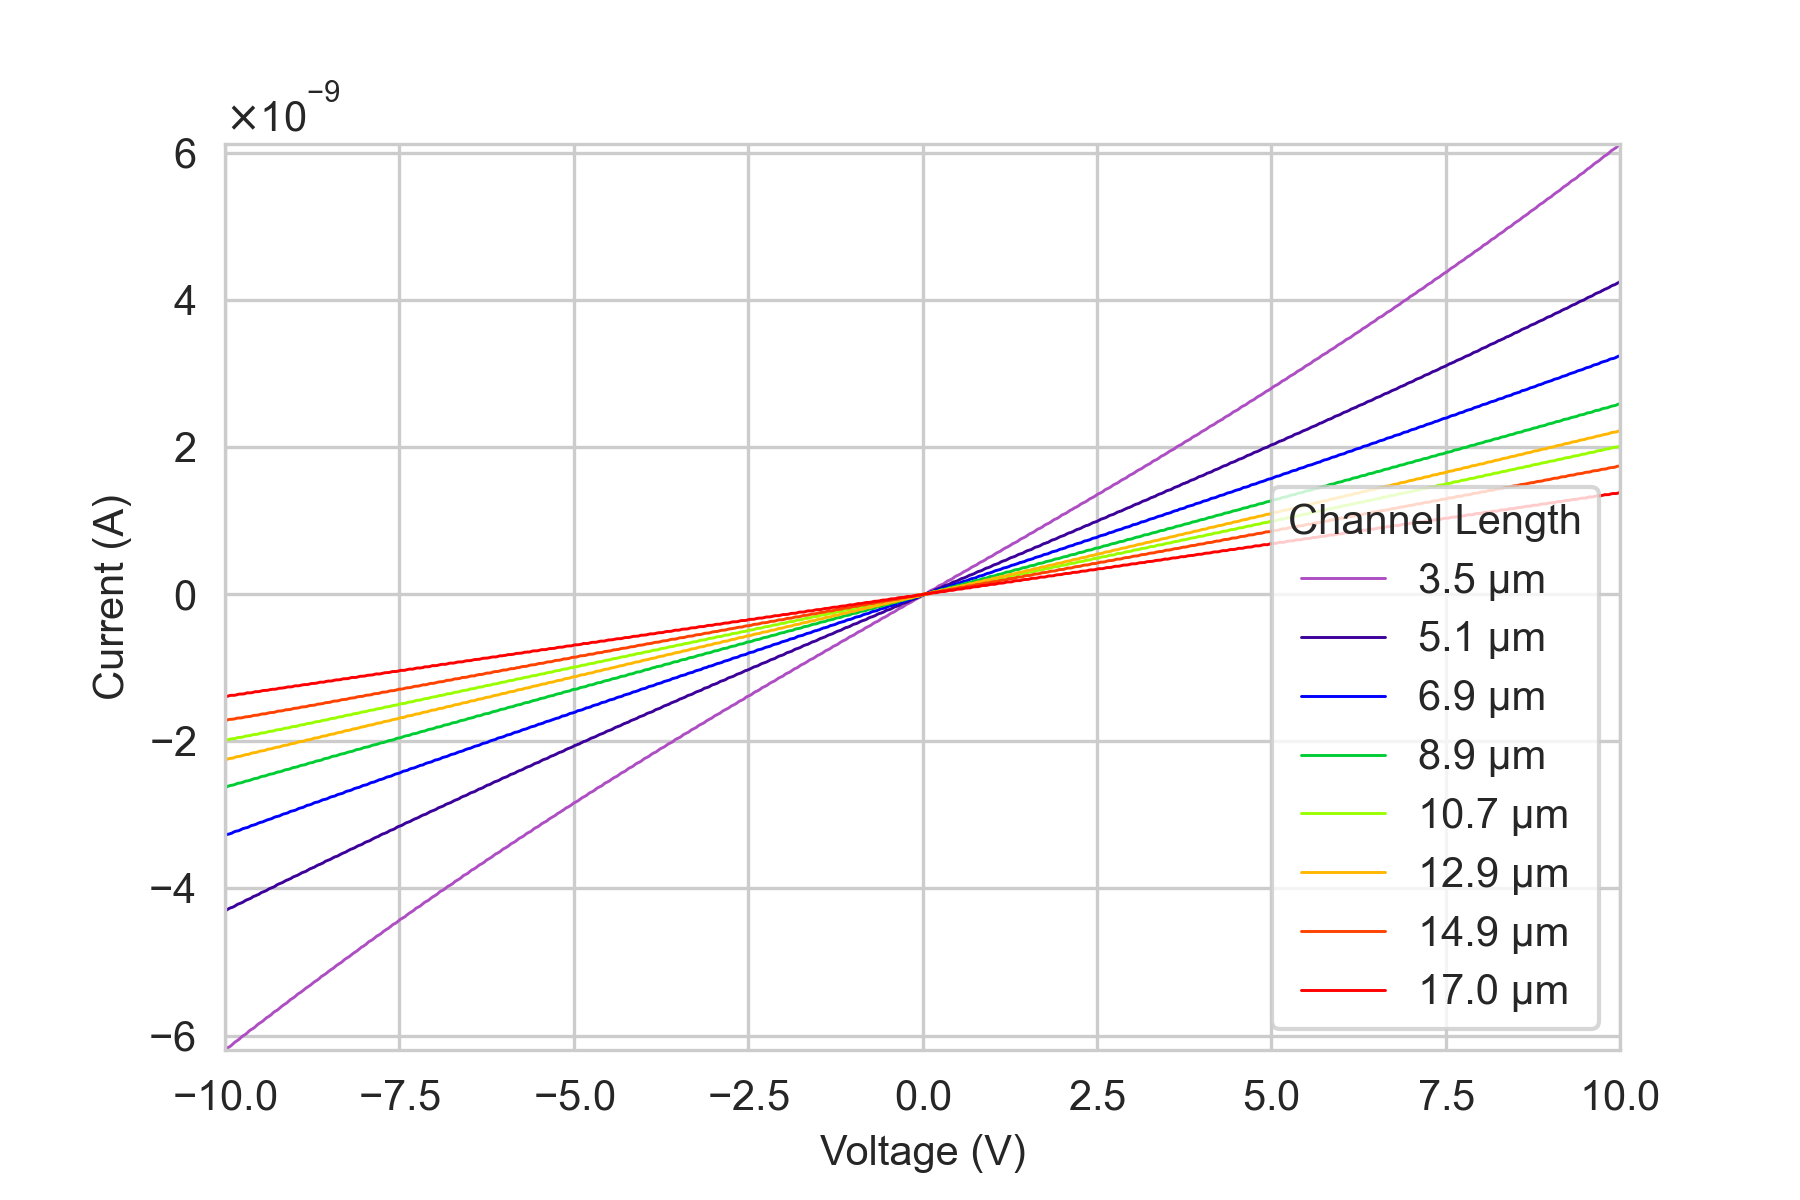
\includegraphics[width=0.97\textwidth]{Chapter6/Figs/Raster/Sample C 2019/IV/10V IV characteristics at 150 C.png}
    \caption{A linear plot of the measured current against applied voltage for all channel lengths at 150\si{\degreeCelsius} (sample C).}
    \label{fig:C_current_voltage_150}
\end{figure}
\begin{figure}[h]
    \centering
    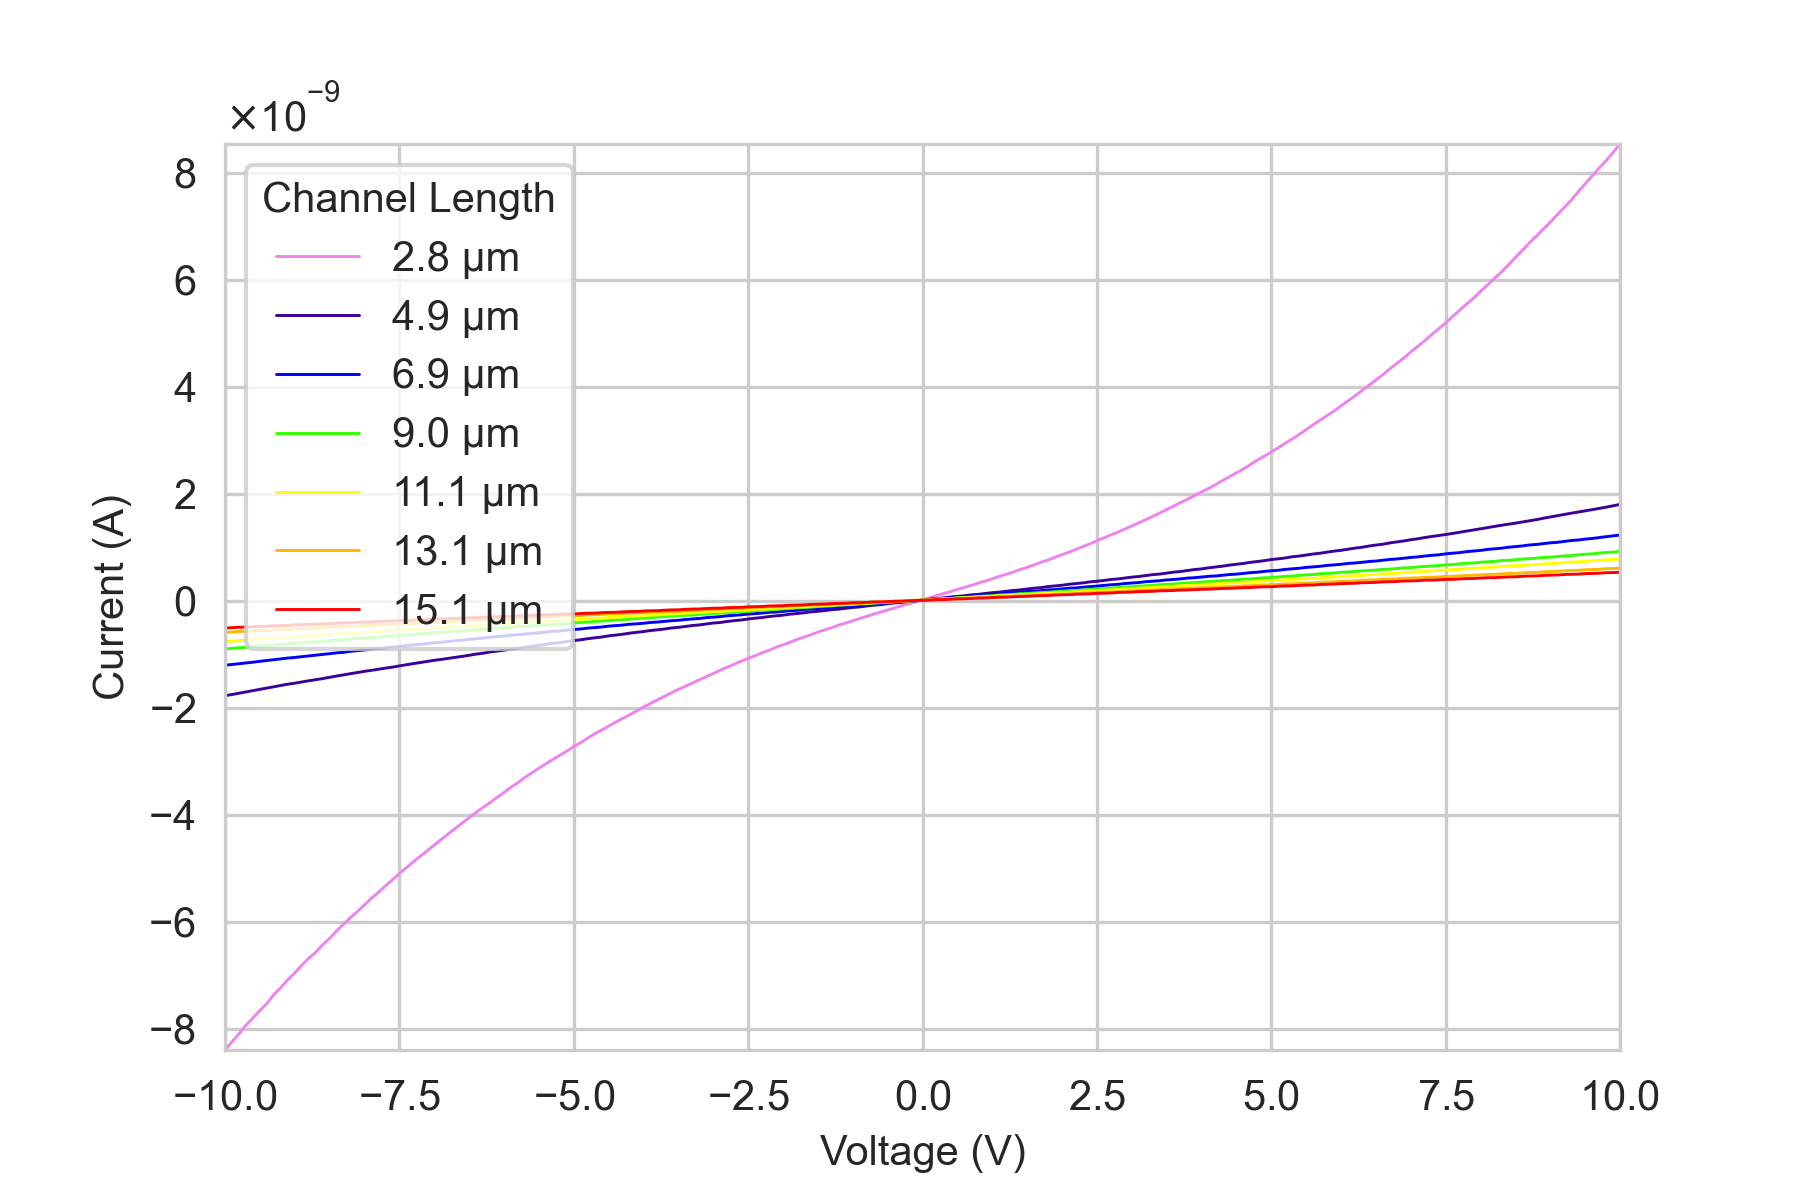
\includegraphics[width=0.97\textwidth]{Chapter6/Figs/Raster/Sample D 2019/IV/10V IV characteristics at 150 C.png}
    \caption{A linear plot of the measured current against applied voltage for all channel lengths at 150\si{\degreeCelsius} (sample D).}
    \label{fig:D_current_voltage_150_10V}
\end{figure}

\begin{figure}[h]
    \centering
    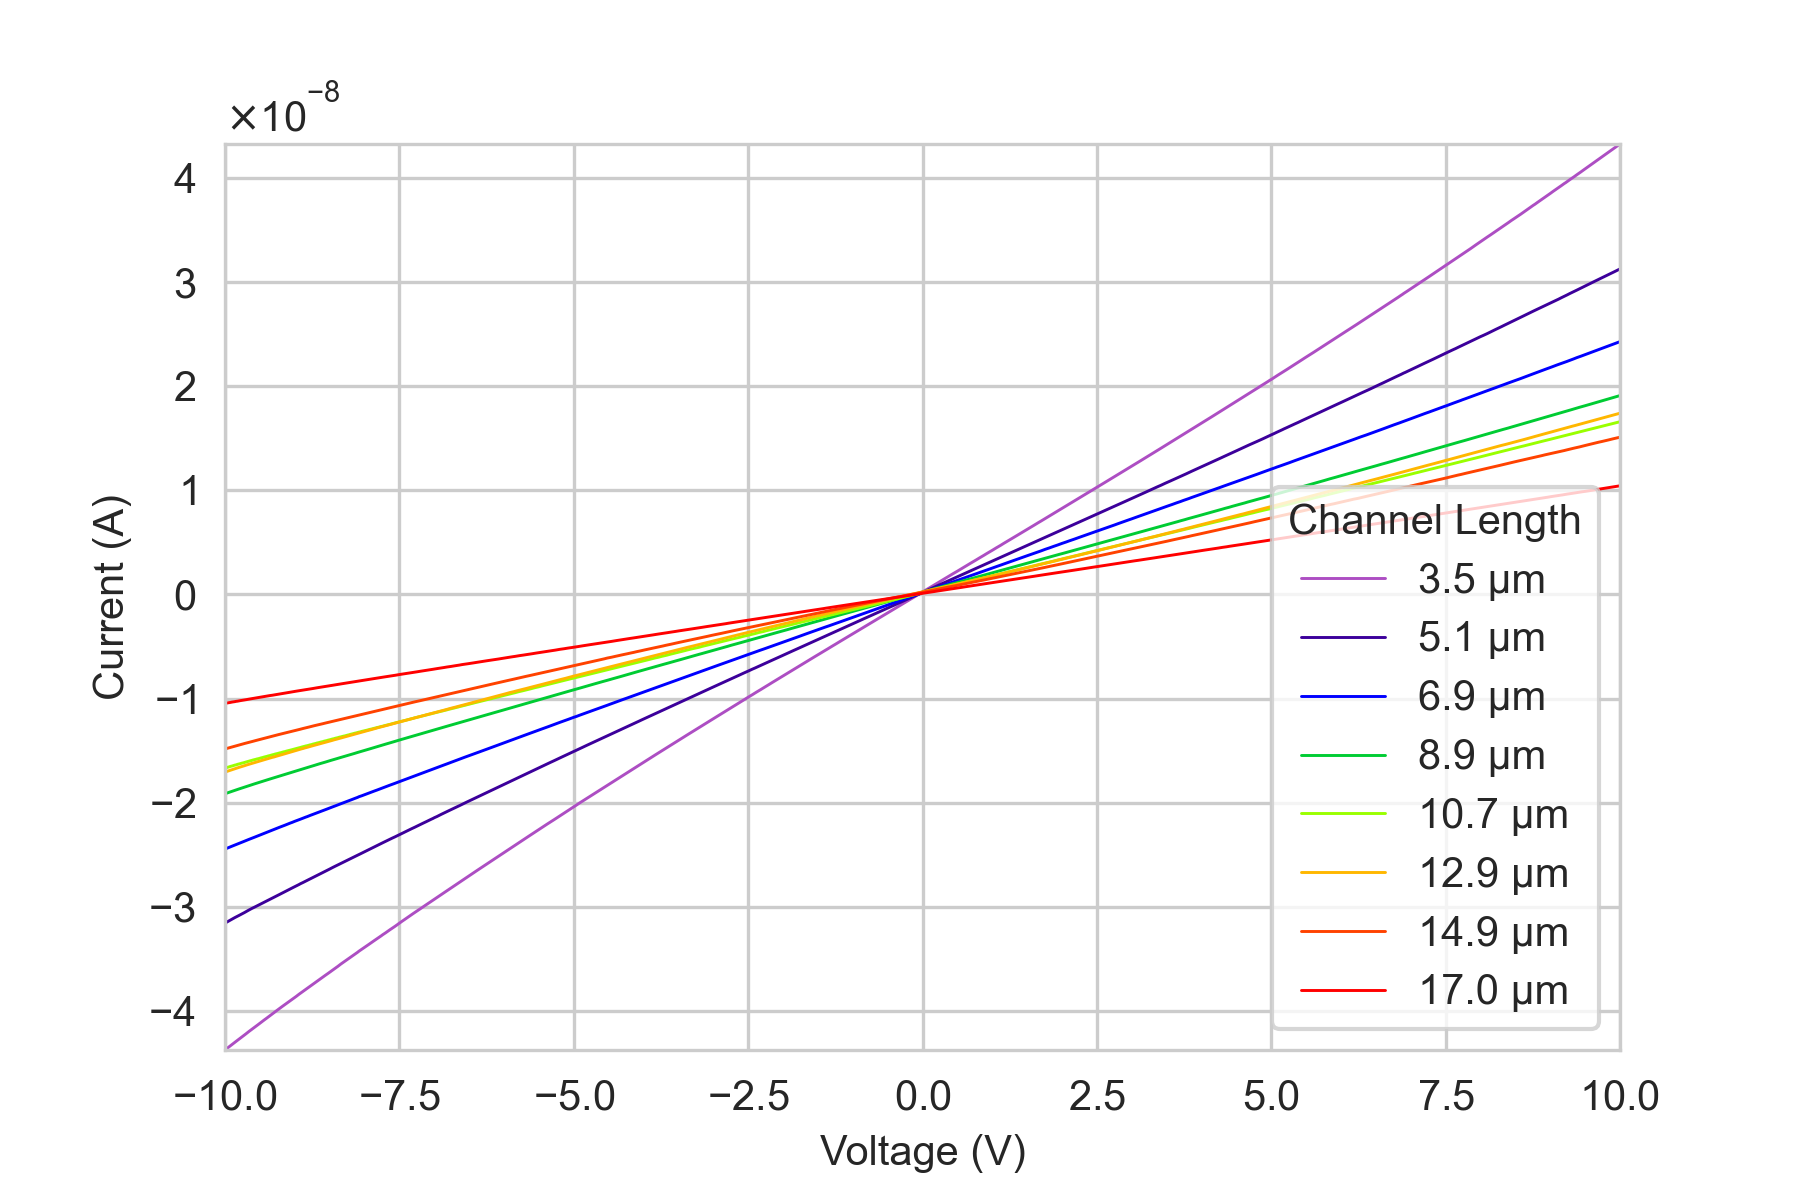
\includegraphics[width=0.97\textwidth]{Chapter6/Figs/Raster/Sample C 2019/IV/10V IV characteristics at 300 C.png}
    \caption{A linear plot of the measured current against applied voltage for all channel lengths at 300\si{\degreeCelsius} (sample C).}
    \label{fig:C_current_voltage_300}
\end{figure}
\begin{figure}[h]
    \centering
    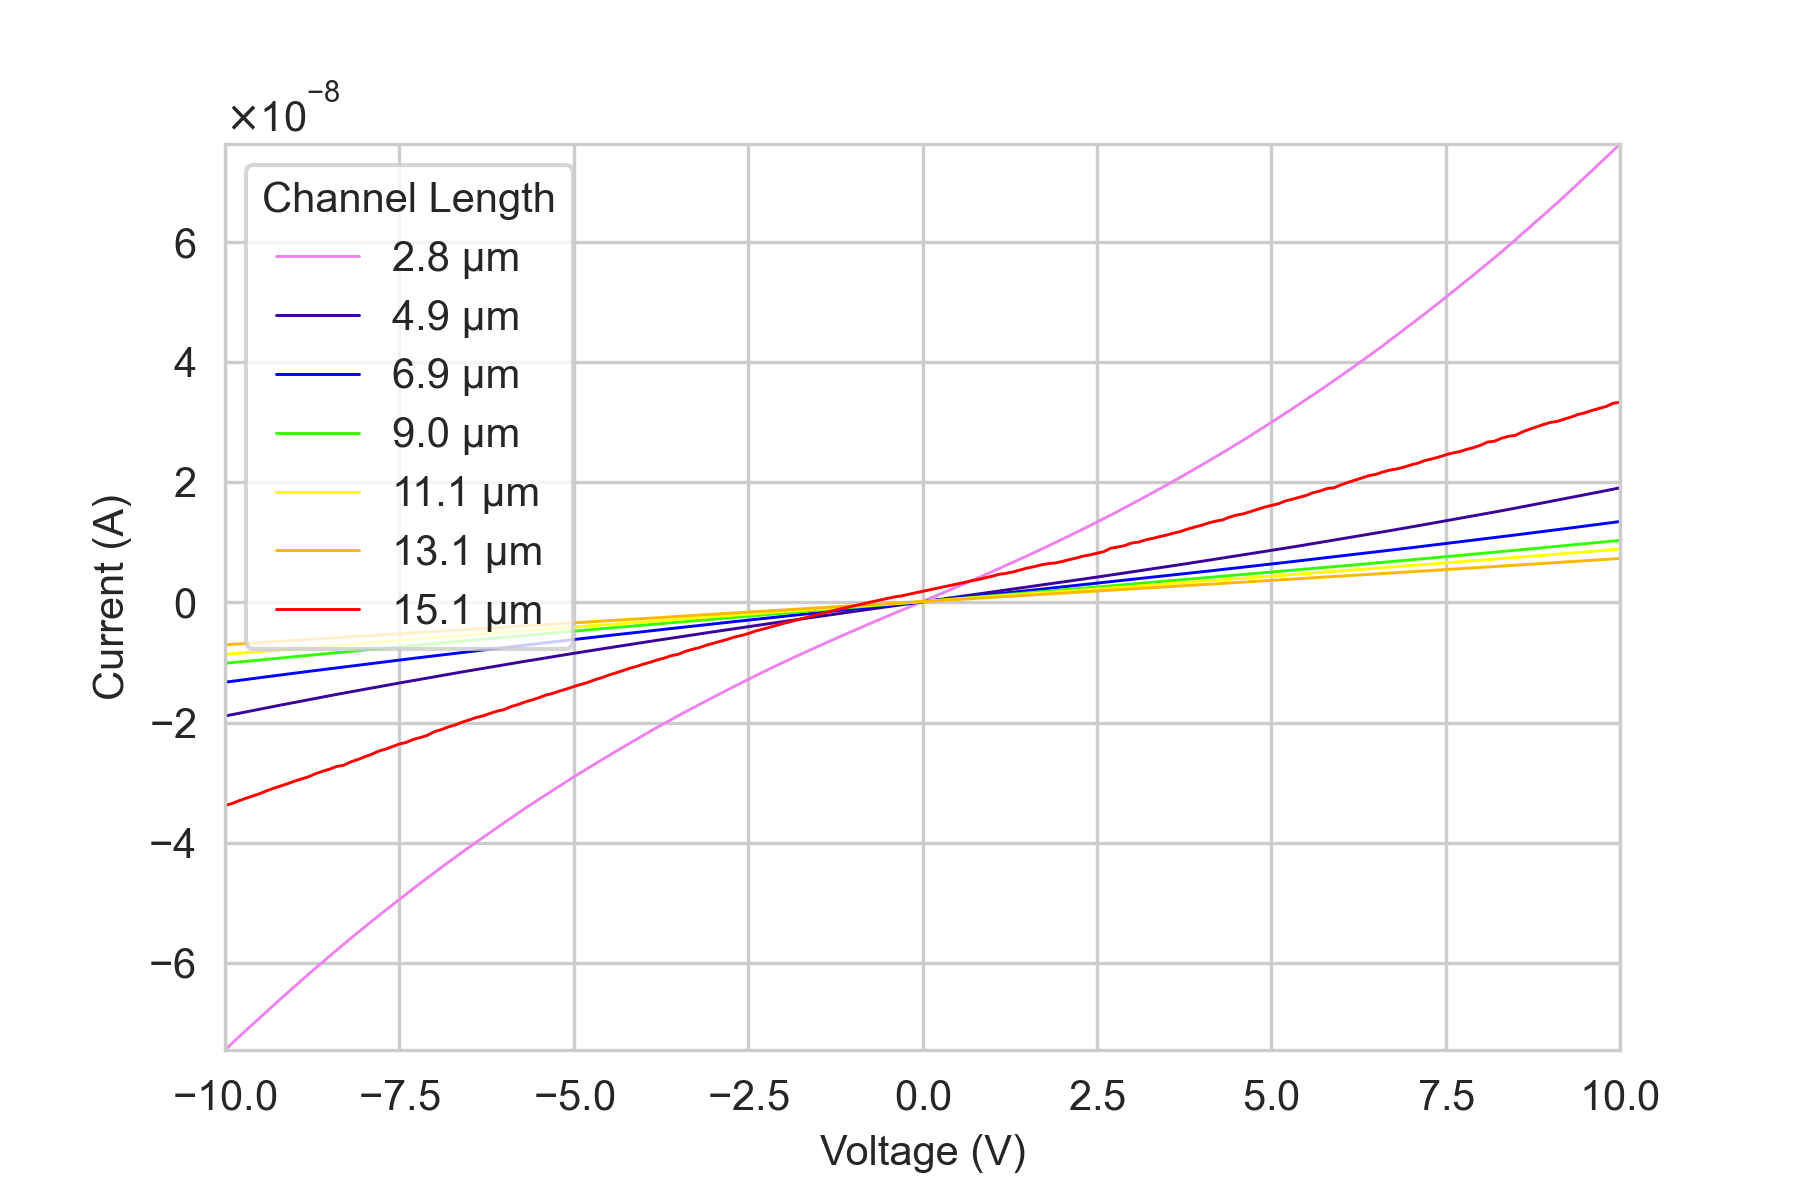
\includegraphics[width=0.97\textwidth]{Chapter6/Figs/Raster/Sample D 2019/IV/10V IV characteristics at 300 C.png}
    \caption{A linear plot of the measured current against applied voltage for all channel lengths at 300\si{\degreeCelsius} (sample D).}
    \label{fig:D_current_voltage_300_10V}
\end{figure}

\FloatBarrier

\subsection{Ti/Pt/Au J-V Results}
This section presents the current density vs applied voltage plots for samples C and D at temperatures of 21, 150, and 300\si{\degreeCelsius}. The bias range used is $\pm10$ \si{\volt}. Error bars representing a current error of $1$ \si{\pico\ampere}, are included in the plots. Data points have been processed using a running average over three consecutive points. For the full set of J-V, please see section \ref{app:LTLM_J_V_data}.

\begin{figure}[h]
    \centering
    \includegraphics[width=0.97\textwidth]{Sample C 2019/10V_Current_Density_vs_Voltage_Temperature_21_log.png}
    \caption{A log-linear plot of the measured current density against applied voltage for all channel lengths at 21\si{\degreeCelsius} (sample C).}
    \label{fig:10V_current_density_21_C}
\end{figure}
\begin{figure}[h]
    \centering
    \includegraphics[width=0.97\textwidth]{Sample D 2019/10V_Current_Density_vs_Voltage_Temperature_21_log.png}
    \caption{A log-linear plot of the measured current density against applied voltage for all channel lengths at 21\si{\degreeCelsius} (sample D).}
    \label{fig:10V__current_density_21_D}
\end{figure}

\begin{figure}[h]
    \centering
    \includegraphics[width=0.97\textwidth]{Sample C 2019/10V_Current_Density_vs_Voltage_Temperature_250_log.png}
    \caption{A log-linear plot of the measured current density against applied voltage for all channel lengths at 150\si{\degreeCelsius} (sample C).}
    \label{fig:10V_current_density_150_C}
\end{figure}
\begin{figure}[h]
    \centering
    \includegraphics[width=0.97\textwidth]{Sample D 2019/10V_Current_Density_vs_Voltage_Temperature_250_log.png}
    \caption{A log-linear plot of the measured current density against applied voltage for all channel lengths at 150\si{\degreeCelsius} (sample D).}
    \label{fig:10V__B_current_density_150_D}
\end{figure}

\begin{figure}[h]
    \centering
    \includegraphics[width=0.97\textwidth]{Sample C 2019/10V_Current_Density_vs_Voltage_Temperature_300_log.png}
    \caption{A log-linear plot of the measured current density against applied voltage for all channel lengths at 300\si{\degreeCelsius} (sample C).}
    \label{fig:10V_current_density_300_C}
\end{figure}
\begin{figure}[h]
    \centering
    \includegraphics[width=0.97\textwidth]{Sample D 2019/10V_Current_Density_vs_Voltage_Temperature_300_log.png}
    \caption{A log-linear plot of the measured current density against applied voltage for all channel lengths at 300\si{\degreeCelsius} (sample D).}
    \label{fig:10V_current_density_300_D}
\end{figure}

\FloatBarrier

\subsubsection{Analysis of J-V Data}
During high-temperature testing of sample D, the electrical characteristics indicated a significant short in the system. Upon investigation, it was discovered that a large flake of the deposited metal had detached from the diamond surface and come into contact with one of the electrical probes during the test procedure. Consultations with Evince Technology indicated that poor adhesion may be a common problem when annealing times significantly exceed 30 minutes. Therefore, the electrical data presented here is that which was measured prior to the flake delamination. However in figure \ref{fig:10V_current_density_300_D}, there is an offset in the position of channel width $15.1$ \si{\micro\metre}, indicating a large error in the system, which is highly likely to be the onset of issues due to delamination. Otherwise, these current density plots show a few clear trends, such as sample D consistently showing higher current than sample C across the $\pm10$ \si{\volt} range. Both samples generally show a clear dependence of the measured current density on the channel widths, indicating higher resistances for increased channel lengths, and the samples show a clear increase of measured current as a function of the temperature, indicating the reduction of resistance via ionisation of deep donors as predicted for phosphorous doped diamond. The same trends can be seen in the linear I-V plots from the previous section.

\subsection{Richardson Plots}
The operating current for an ideal Schottky diode under a forward bias where $qV > 3kT$, based on the thermionic emission of electrons, is given by \cite{sze2006} as:
\begin{equation}
    I=I_{s}\exp{qV/nkT}\left[1-\exp{-qV/kT}\right]
\end{equation}
Where $I_{s}$ is the saturation current, $q$ is the elementary charge, $V$ is the applied voltage, $n$ is the diode ideality factor, $k$ is the Boltzmann constant and $T$ is the temperature. In this ideal case, the carrier conduction in a forward bias is dominated by the thermal emission of carriers from the semiconductor over a spatially homogenous barrier into the metal. This equation can be rearranged into a format that allows for a graphical analysis:

\begin{equation}
    \ln{\frac{I}{1-\exp{\left(-\beta V\right)}}} = \frac{\beta V}{n} + \ln{I_{s}}
    \label{eq:thermionic_emission_graphical}
\end{equation}

Here, \(\beta=\frac{q}{kT}\). The saturation current $I_{s}$ is given by:

\begin{equation}
    \ln{\frac{I_{s}}{AT^{2}}} = -q\frac{\Phi_{Beff}}{kT} + \ln{A^{*}_{eff}}
\end{equation}

Where $A^{*}_{eff}$ is the effective Richardson constant, $A$ is the area of the Schottky contact and $\Phi_{Beff}$ is the effective barrier height. The Richardson constant, \( A^{*} \), which characterises the thermionic emission process, arises from the Richardson-Dushman equation for thermionic emission. For an in-depth definition of this constant in the context of thermionic emission theory, please see section \ref{sec:thermionic_emission_theory}.

In practice, \( A \) can vary for different materials. For instance, in polycrystalline metals, \( A \) can range from about \SI{32}{\ampere\per\centi\meter\squared\per\kelvin\squared} to \SI{160}{\ampere\per\centi\meter\squared\per\kelvin\squared} and can vary even more widely for oxide and composite surfaces. The theoretical value of the Richardson constant is

\begin{equation}
    A^{*} = \frac{4\pi qk^{2}m^{*}}{h^{3}}
\end{equation}

Where:
\begin{itemize}
    \item \(m^{*}\): Effective electron mass
    \item \(h\): Planck's constant
\end{itemize}

\begin{figure}[h]
    \centering
    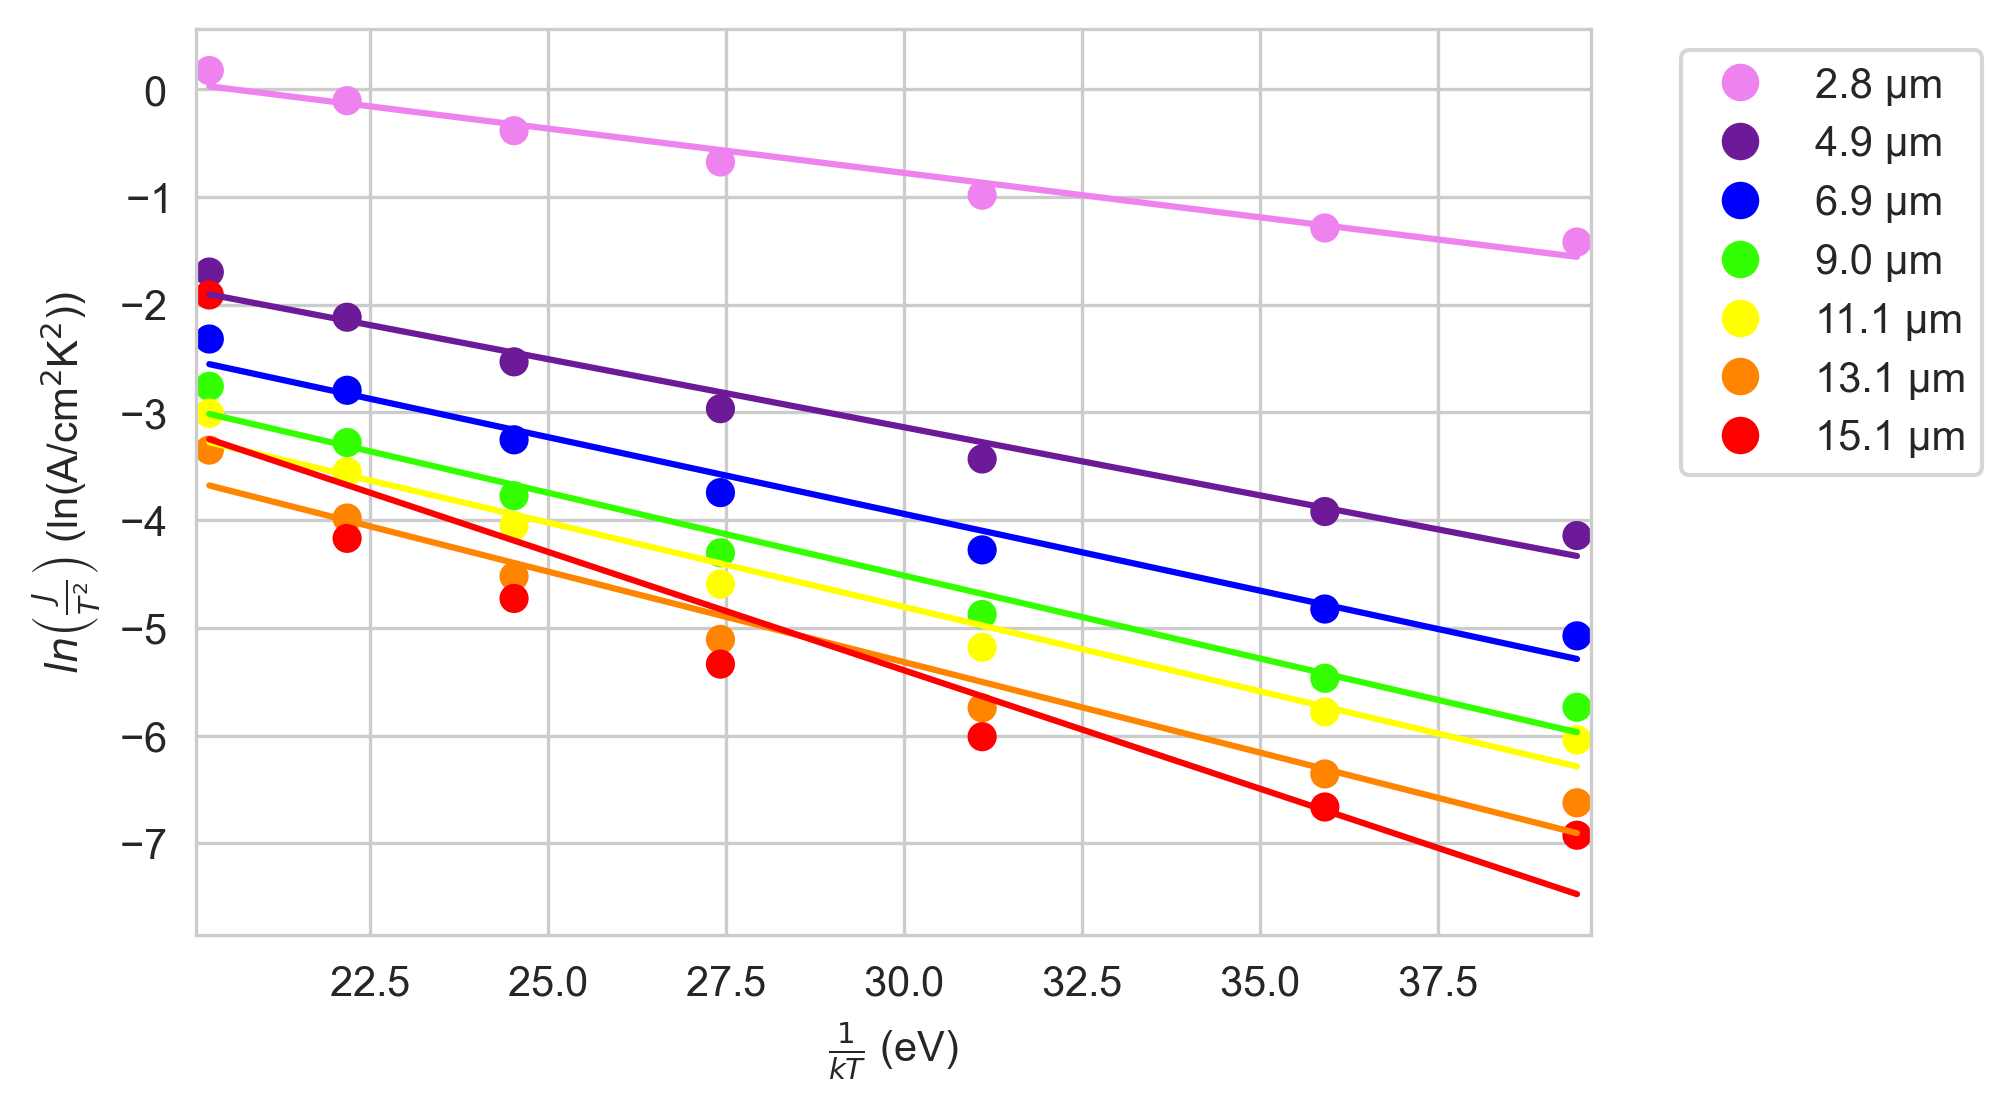
\includegraphics[width=\textwidth]{Sample C 2019/Richardson_Plot.png}
    \caption{A conventional Richardson plot for the various channel widths tested (Sample C, 10V range).}
    \label{fig:richardsonC}
\end{figure}

\begin{table}[h]
    \centering
    \begin{tabular}{|c|c|c|c|c|}
        \hline
        Channel (\si{\micro\metre}) & Barrier (\si{\electronvolt}) & Diff. from Mean (\si{\electronvolt}) & $A*_{eff}$ (\si{\ampere\per\centi\metre\squared\per\kelvin\squared}) & $R^{2}$\\ \hline
        3.529 & 0.1515 & -0.0090 & 1.53e+07 &0.9888 \\ 
        5.064 & 0.1565 & -0.0040 & 1.22e+07 &0.9892 \\ 
        6.949 & 0.1576 & -0.0029 & 9.62e+06 &0.9884 \\ 
        8.947 & 0.1599 & -0.0006 & 8.10e+06 &0.9918 \\ 
        10.720 & 0.1595 & -0.0010 & 6.75e+06 &0.9865 \\ 
        12.890 & 0.1709 & 0.0104 & 8.96e+06 &0.9889 \\ 
        14.930 & 0.1669 & 0.0064 & 6.75e+06 &0.9876 \\ 
        16.970 & 0.1615 & 0.0010 & 4.51e+06 &0.9900 \\ 
        \hline
    \end{tabular}
    \caption{Extracted parameters from the Richardson plot for sample C.}
    \label{tab:richardsonC}
\end{table}
\begin{figure}
    \centering
    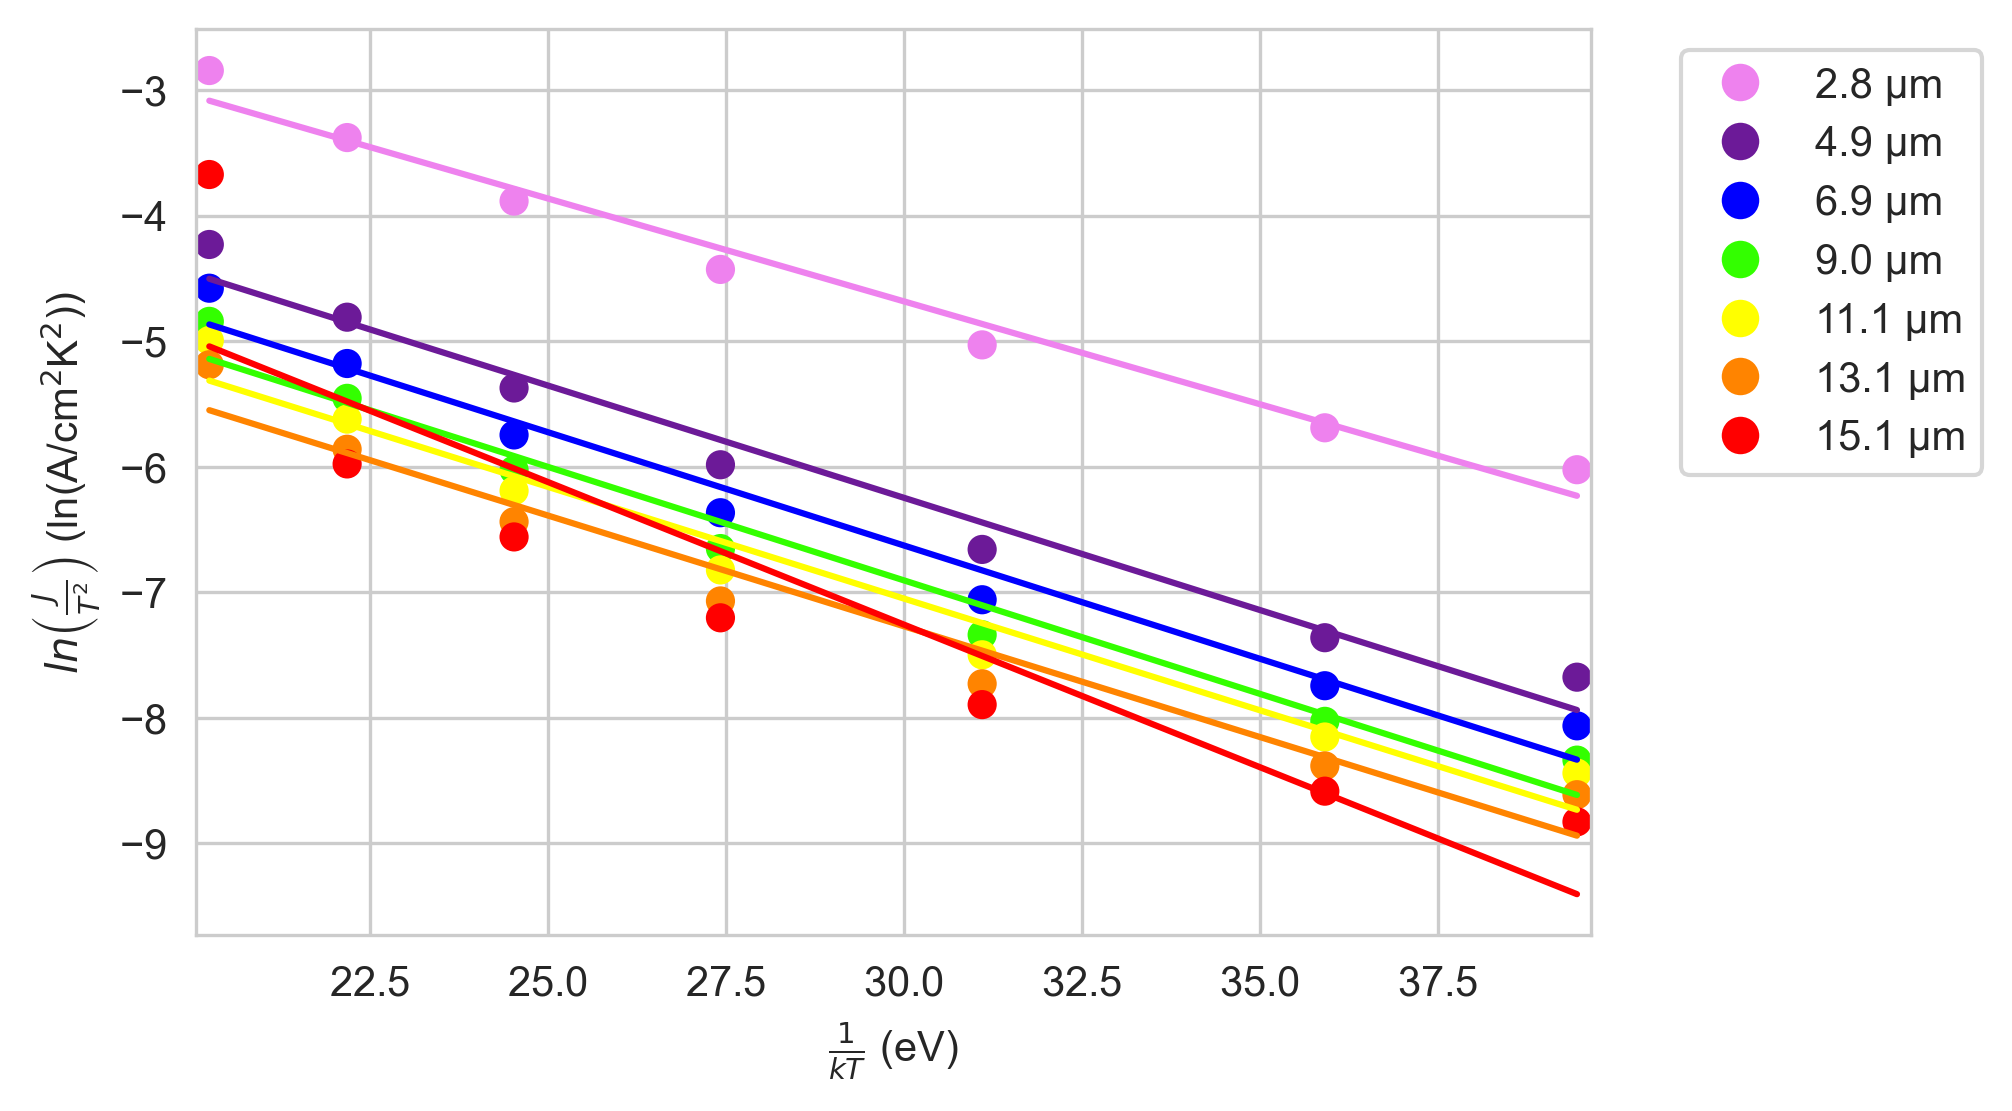
\includegraphics{Chapter6/Figs/Raster/Sample D 2019/10V_Richardson_Plot.png}
    \caption{A conventional Richardson plot for the various channel widths tested (Sample D, 10 V range).}
    \label{fig:enter-label}
\end{figure}

\begin{table}[h]
    \centering
    \begin{tabular}{|c|c|c|c|c|}
        \hline
        Channel (\si{\micro\metre}) & Barrier (\si{\electronvolt}) & Diff. from Mean (\si{\electronvolt}) & $A*_{eff}$ (\si{\ampere\per\centi\metre\squared\per\kelvin\squared}) & $R^{2}$\\ \hline
        2.803 & 0.1639 & -0.0198 & 3.16e+07 &0.9799 \\ 
        4.862 & 0.1789 & -0.0048 & 1.04e+07 &0.9757 \\ 
        6.945 & 0.1806 & -0.0031 & 7.44e+06 &0.9739 \\ 
        9.029 & 0.1809 & -0.0028 & 5.69e+06 &0.9725 \\ 
        11.110 & 0.1780 & -0.0057 & 4.52e+06 &0.9679 \\ 
        13.150 & 0.1765 & -0.0072 & 3.46e+06 &0.9603 \\ 
        15.130 & 0.2272 & 0.0435 & 1.61e+07 &0.8324 \\ 
        \hline
    \end{tabular}
    \caption{Extracted parameters from the Richardson plot for sample D.}
    \label{tab:richardsonD_10V}
\end{table}

\begin{figure}[h]
    \centering
    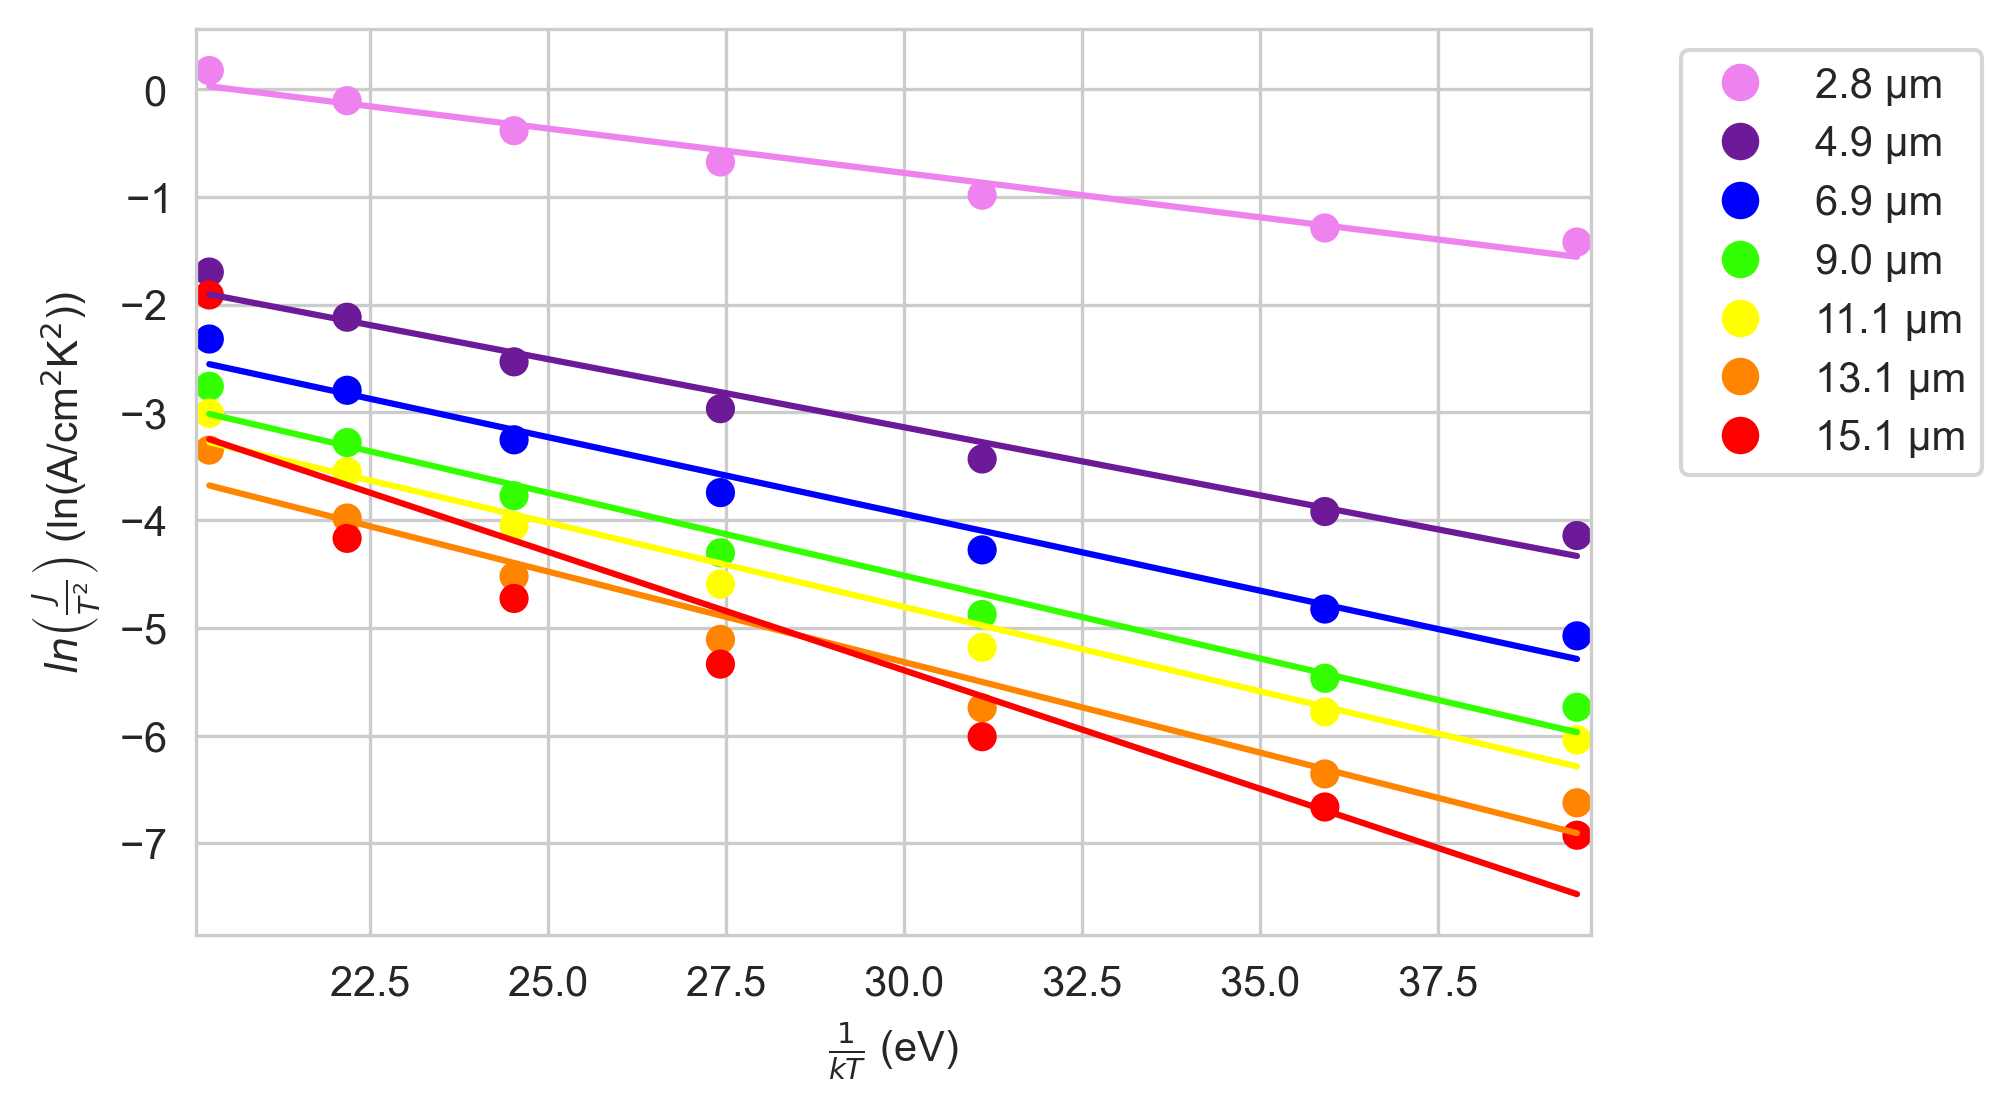
\includegraphics[width=\textwidth]{Sample D 2019/50V_Richardson_Plot.png}
    \caption{A conventional Richardson plot for the various channel widths tested (Sample D, 50 V range).}
    \label{fig:richardsonD_50V}
\end{figure}

\begin{table}[h]
    \centering
    \begin{tabular}{|c|c|c|c|c|}
        \hline
        Channel (\si{\micro\metre}) & Barrier (\si{\electronvolt}) & Diff. from Mean (\si{\electronvolt}) & $A*_{eff}$ (\si{\ampere\per\centi\metre\squared\per\kelvin\squared}) & $R^{2}$\\ \hline
        2.803 & 0.0824 & -0.0676 & 1.36e+08 &0.9670 \\ 
        4.862 & 0.1265 & -0.0235 & 4.83e+07 &0.9729 \\  
        6.945 & 0.1425 & -0.0075 & 3.49e+07 &0.9731 \\ 
        9.029 & 0.1539 & 0.0039 & 2.77e+07 &0.9727 \\ 
        11.110 & 0.1567 & 0.0067 & 2.25e+07 &0.9710 \\ 
        13.150 & 0.1681 & 0.0181 & 1.90e+07 &0.9651 \\ 
        15.130 & 0.2200 & 0.0700 & 8.35e+07 &0.8304 \\ 
        \hline
    \end{tabular}
    \caption{Extracted parameters from the Richardson plot for sample D.}
    \label{tab:richardsonD_50V}
\end{table}

To examine the method of electron emission from the contacts, a conventional Richardson plot is shown in figures \ref{fig:richardsonC} and \ref{fig:richardsonD} for a constant bias range of $\pm10$ \si{\volt}. By fitting a linear relationship to this data, as according to equation \ref{eq:thermionic_emission_graphical}, the average Schottky barrier height for samples C and D is extracted to be 0.161 \si{\electronvolt} and 0.150 \si{\electronvolt}, with a standard deviation of $5.56\times10^{-3}$ \si{\electronvolt} and $3.86\times10^{-2}$ \si{\electronvolt}, respectively. The exact results as determined from linear lines of best fit are shown in tables \ref{tab:richardsonC} and \ref{tab:richardsonD}.

\begin{figure}[htbp]
    \centering
    \begin{subfigure}[b]{0.49\textwidth}
        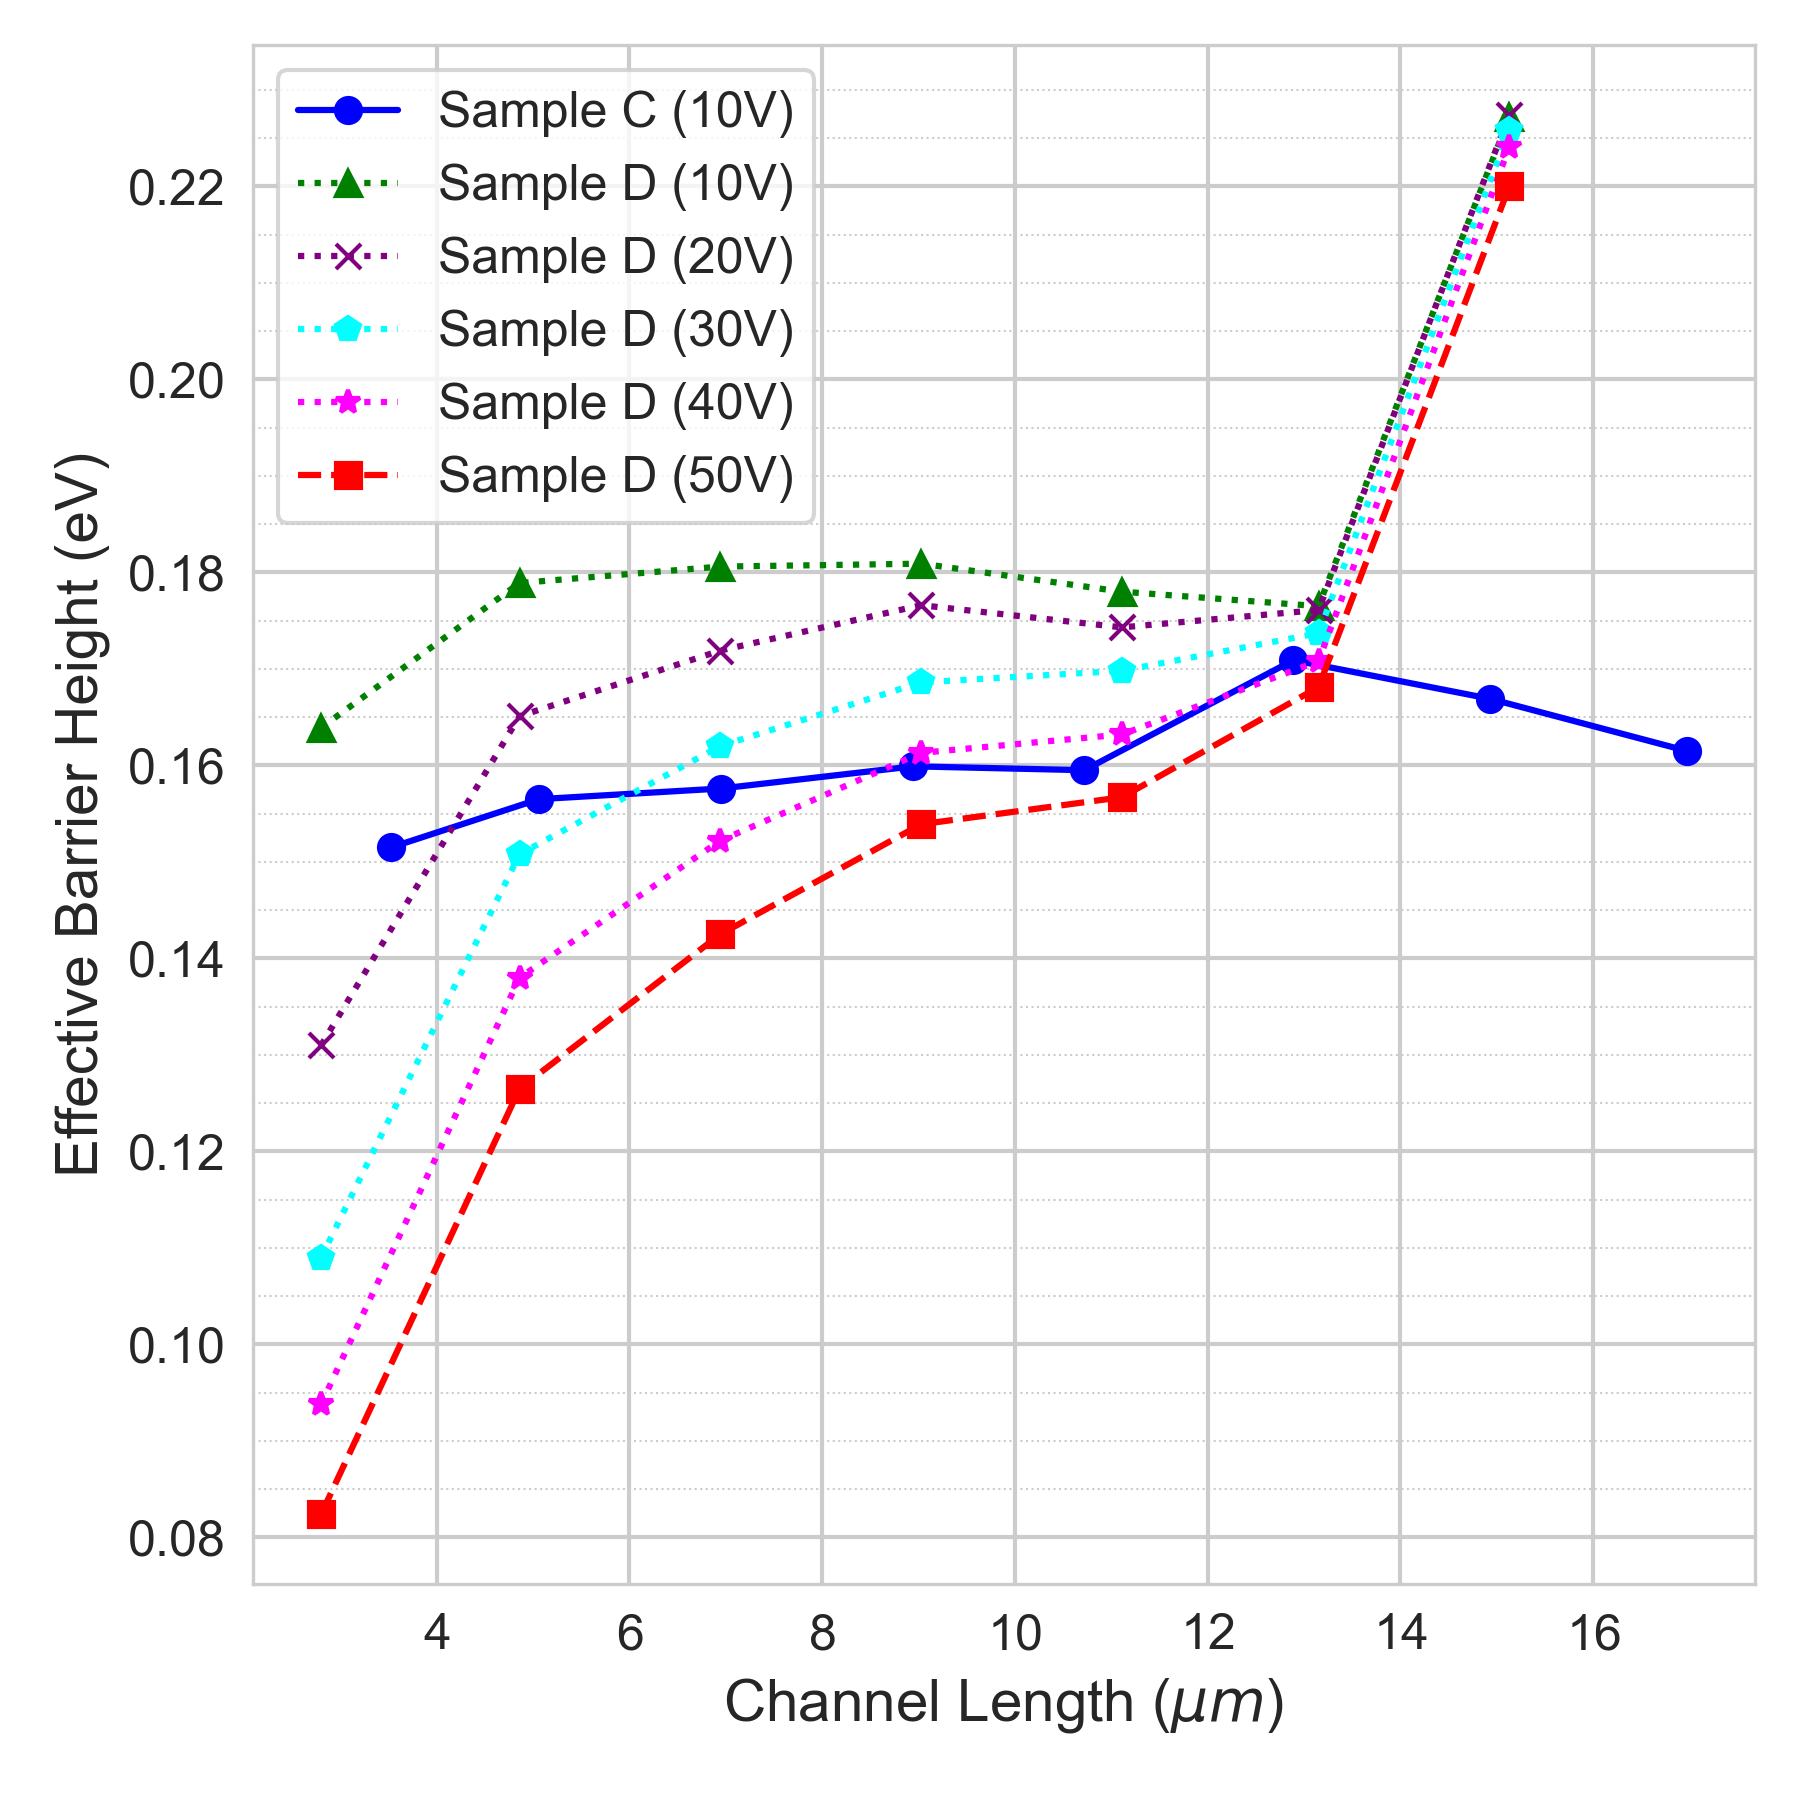
\includegraphics[width=\textwidth]{Chapter6/Figs/Raster/barrier_comparison.png}
        \caption{The measured values for the barrier heights as a function of the linear TLM channel length.}
        \label{fig:barrier}
    \end{subfigure}
    \hfill % Spaces the figures a bit
    \begin{subfigure}[b]{0.49\textwidth}
        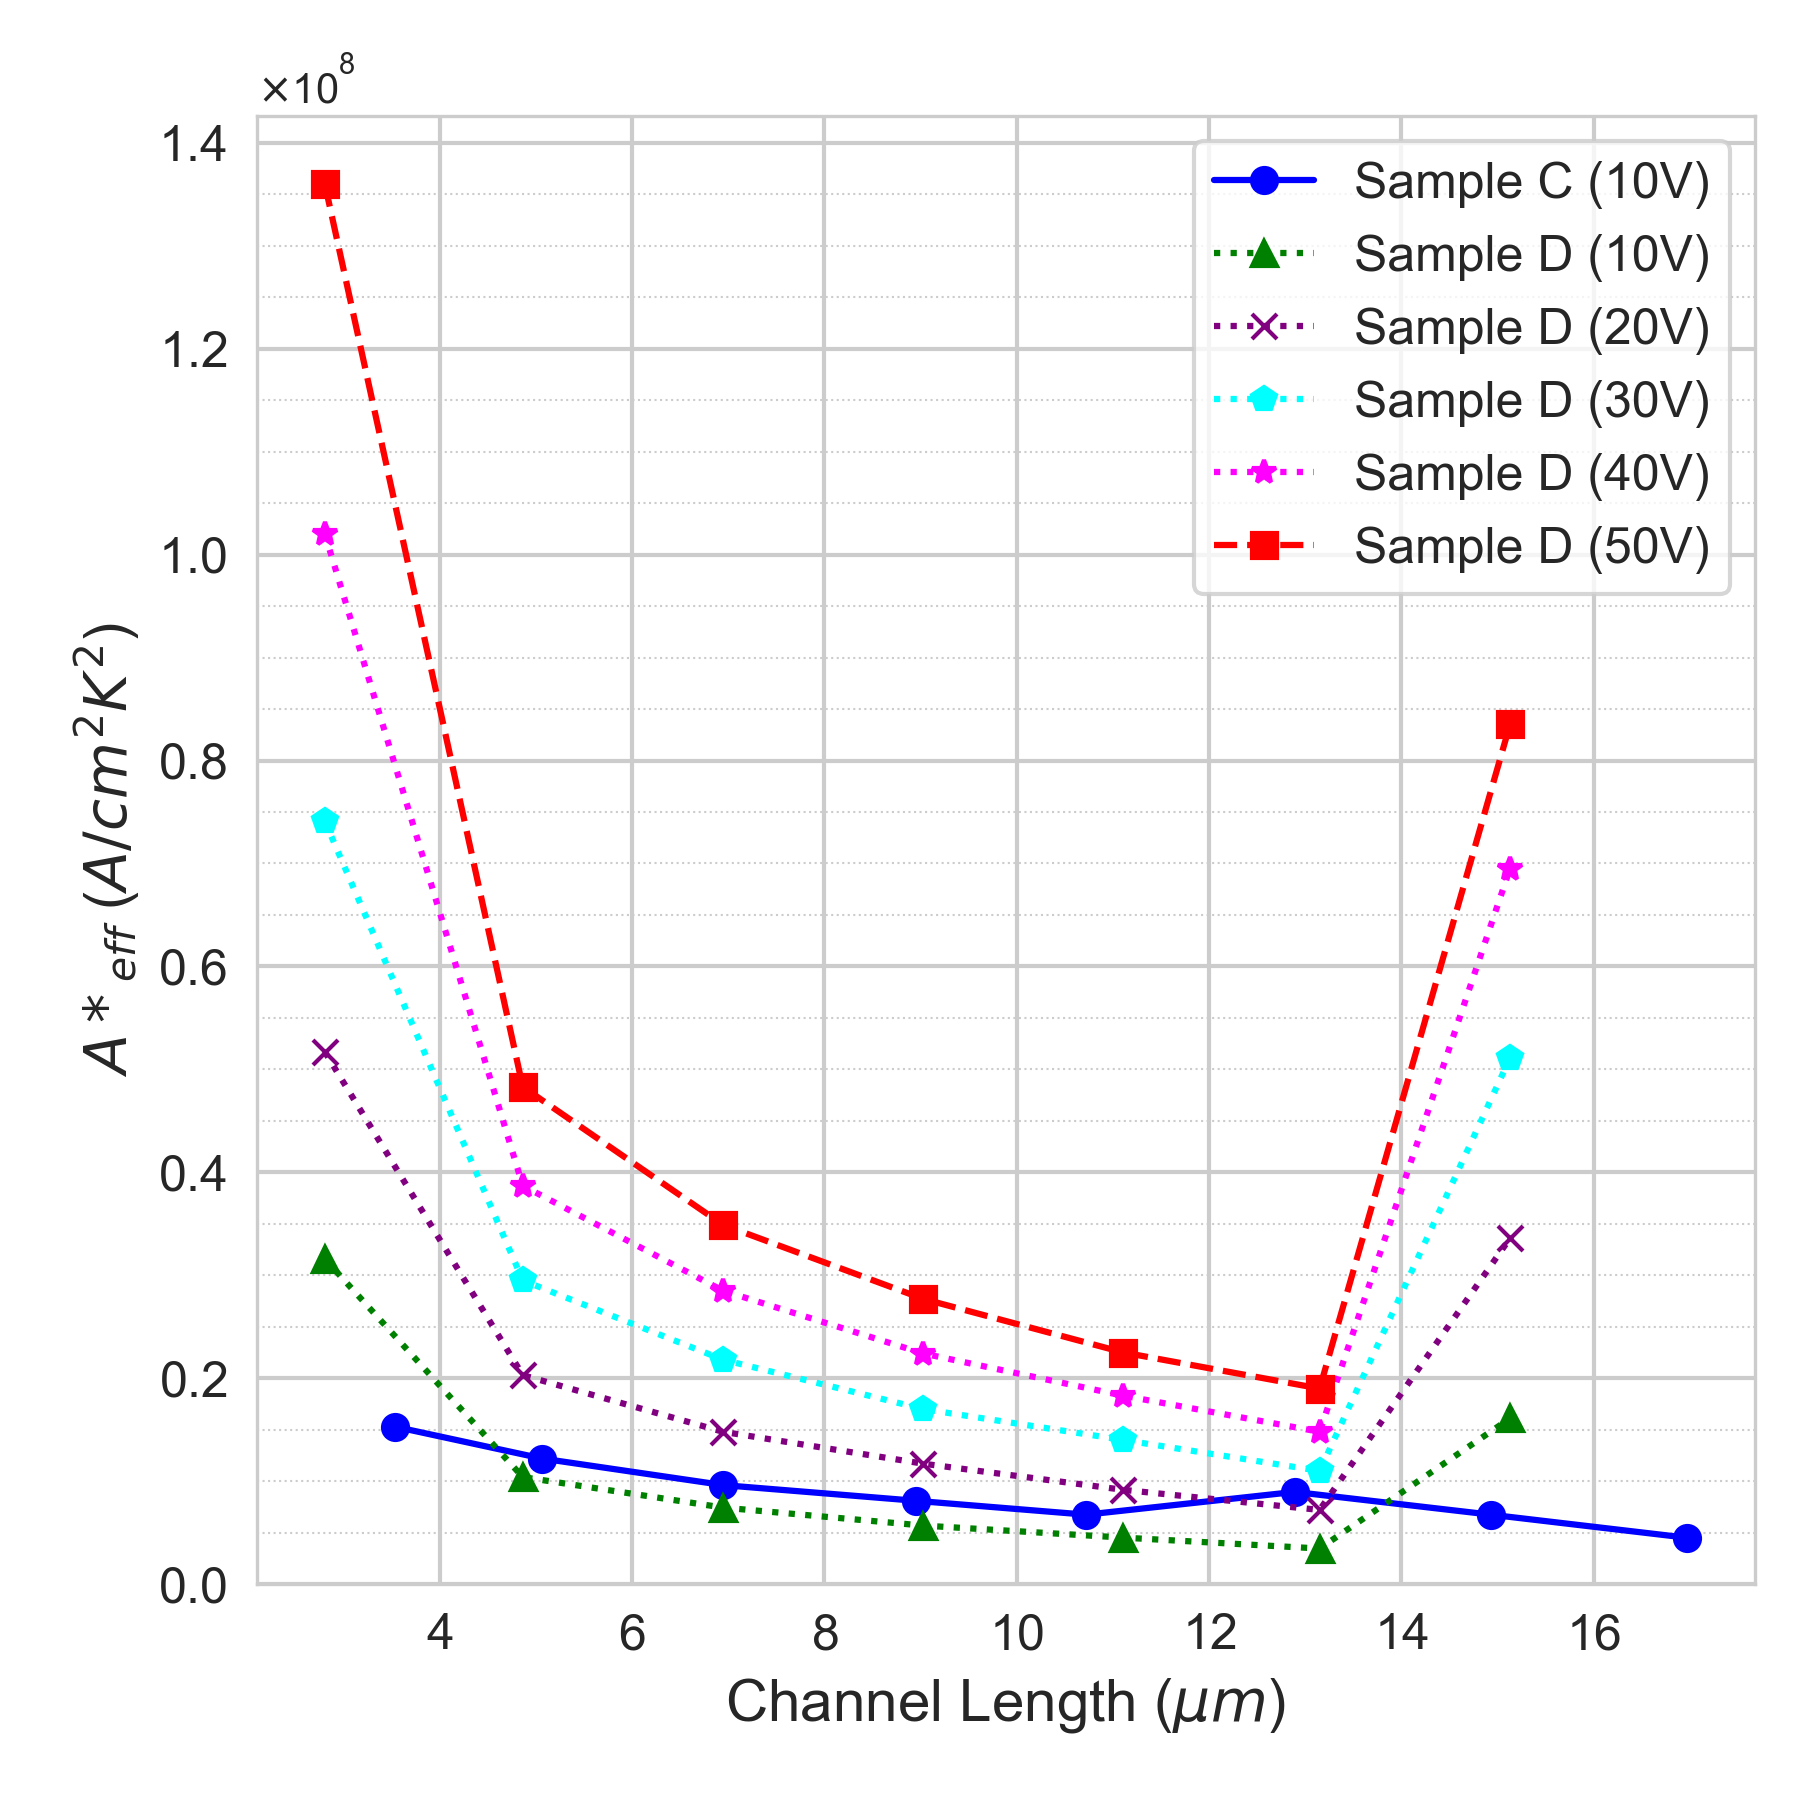
\includegraphics[width=\textwidth]{Chapter6/Figs/Raster/richardson_comparison.png}
        \caption{The measured values for the Richardson constant as a function of the linear TLM channel length.}
        \label{fig:richardson}
    \end{subfigure}
    \caption{(a) Effective barrier height vs. linear TLM channel length. (b) Effective Richardson constant vs. linear TLM channel length.}
    \label{fig:side_by_side_barrier_richardson}
\end{figure}

 One observation from this data is that sample C displayed a relatively constant barrier height, regardless of the channel length, while sample D shows a proportionality between the channel length and the effective barrier height. This could be due to the difference in the smallest channel sizes. While both sets of metal contacts were formed with the same shadow mask in the process of metal deposition via photolithography, the as formed contacts had a measurably different channel length at the smallest scales. The smallest channel as measured via AFM on sample C was $3.5$ \si{\micro\metre}, while sample D had a channel length of $\approx2.8$ \si{\micro\metre}. 
 
 The smallest channel of sample D presents an effective barrier height of $\approx0.08$ \si{\electronvolt}, while the largest channel was $\approx0.22$ \si{\electronvolt}. Similarly, there is an inverse proportionality between the channel length and the observed Richardson constant for both samples, with sample C's Richardson constant consistently an order of magnitude greater than sample D. This is shown in figure \ref{}


\subsection{XPS Analysis}

Further to the SIMS analysis of films grown for one hour, XPS measurements were performed on a sample that had been used for a four hour deposition of highly phosphorous doped material. Additional samples included in this batch of doped diamond growth were used for circular-TLM measurements. The growth duration was chosen to be 4 hours based on the previous observation via SIMS of a growth rate of 0.3 \si{\micro\metre\per\hour}, with the aim being the production of a $\approx1$ \si{\micro\metre} thick surface layer. This would ensure that any conduction measured through the phosphorous doped diamond film would be comparable to other work in this area, with bulk conduction instead of conduction through nanometre scale material.

\section{Circular Transfer Length Method (CTLM)}
\subsection{CTLM Theory}
\begin{figure}[h]
    \centering
    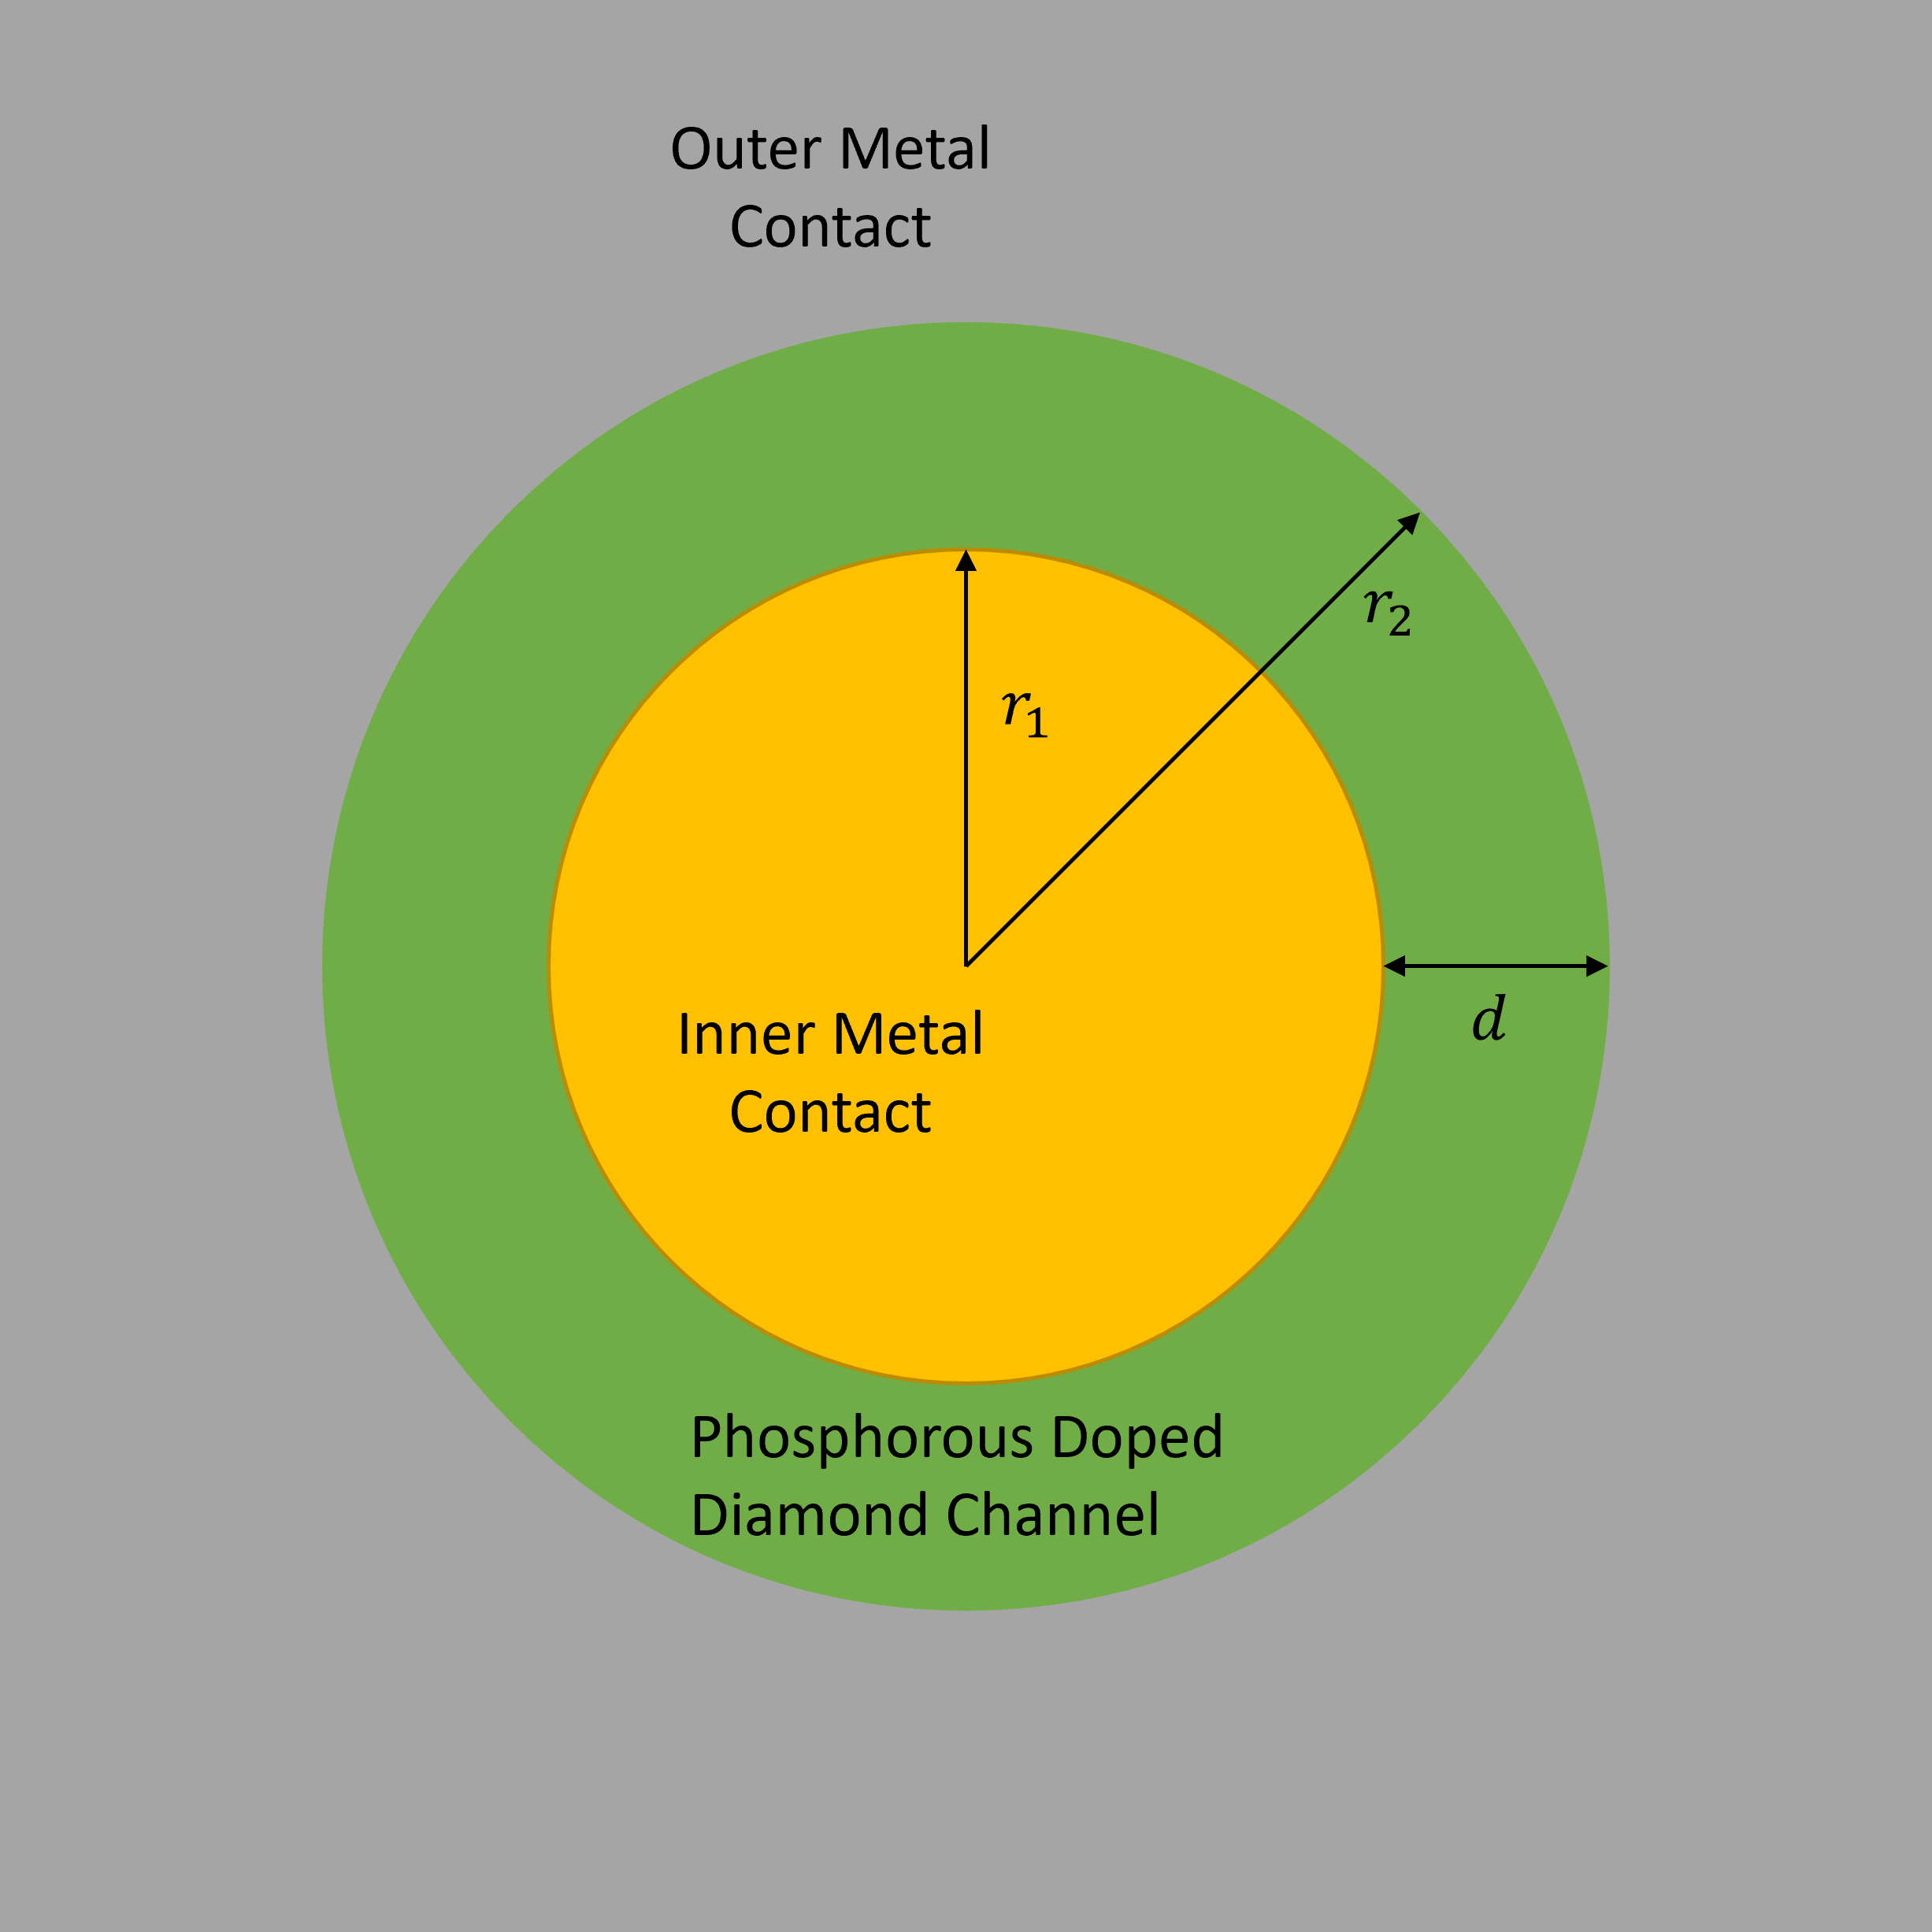
\includegraphics[width=0.7\textwidth]{Chapter6/Figs/Raster/CTLM design.png}
    \caption{The CTLM structure as used in this work.}
    \label{fig:ctlm_structure}
\end{figure}
Generally, the total resistance in CTLM is given by:
\begin{equation}
    R_{T} = \frac{\rho_{s}}{2\pi} \left(L_{T}\left(\frac{1}{r_{1}}+\frac{1}{r_{2}}\right)+\ln{\frac{r_{2}}{r_{1}}}\right)
    \label{eq:ctlm_theory}
\end{equation}
where $\rho_{s}$ is the sheet resistance of the semiconductor layer and $L_{T}$ is the transfer length. $L_{T}$ gives the specific contact resistance $\rho_{c}$ with $L_{T}=\sqrt{\frac{\rho_{c}}{\rho_{s}}}$. When the inner and outer electrode radii $r_{1}+r_{2}$ are constant, depicted by figure \ref{fig:ctlm_structure}, the inner radius is given by:
\begin{equation}
    r_{1} = r_{0} - \frac{d}{2}
\end{equation}
and the outer radius similarly is given by:
\begin{equation}
    r_{2} = r_{0} + \frac{d}{2}
\end{equation}
allowing for the total resistance $R_{T}$ between circular electrodes to follow a linear relationship to the spacing ($d$) of said electrodes:
\begin{equation}
    d = r_{2} - r_{1}
\end{equation}
this then allows for the fitting of measured $R_{T}$ for different spacings $d$ to extract $\rho_{s}$ and $L_{T}$ via equation \ref{eq:ctlm_theory}. Therefore, the total resistance measured can be split into that of the bulk resistance which depends directly on $d$ and the contact resistance independent of $d$, calculating the specific contact resistance $\rho_{c}$. 

One of the key advantages of CTLM theory over LTLM is that of simplicity in fabrication. LTLM structures rely primarily upon etching of material to form "mesa steps", which then prevent the leakage of current around the channel formed between adjacent contacts. While this has been performed for diamond characterisation via inductively coupled plasma etching (ICP) \cite{defeudis2019}, it is also common practice to instead rely upon alternative geometric structures which do not allow for leakage current to flow around that of the specified channels, such as in the case of circular contacts. With two concentric rings as electrical contacts, the channel length between any two nearest points of the contacts remains that of the intended channel length, with no fringe effect paths available.
\subsection{Double Schottky CTLM}
Further to the general CTLM theory, consideration must also be given to the double Schottky nature of these contacts, due to the Fermi-level pinning of metal contacts on the diamond surface. As discussed further in earlier chapters, this maintains a Schottky barrier despite careful selection of metal work functions and carbide formation via annealing. In many early publications which examine this topic in the case of phosphorous doped diamond and the formation of metal contact to such substrates, the voltage ranges examined are large enough to significantly reduce the impact of this barrier on a typical IV plot. It is only in the lower voltage ranges, where the specific contact resistance is a significant parasitic power draw that these Fermi-level pinned Schottky barriers produce a large effect. 

When the resulting double Schottky structure is applied to CTLM theory, the contact resistance $R_{c}$ includes a nonlinear term $R_{N}$ and the conventional linear term of $R_{L}$. This can also be expressed as the nonlinear voltage $V_{N}$ Expressed as a function $V$ of the current $I$:
\begin{equation}
    V(I) = R_{C}I + R_{bulk}I = R_{L}I + V_{N}(I) + V_{N}(-I) + R_{bulk}I
\end{equation}
where $R_{bulk} = \rho_{s}\frac{d}{2\pi r_{0}}$ is the bulk resistance of the doped semiconductor layer and the term $R_{L} = \rho_{s}\frac{2L_{L}}{2\pi r_{0}}$ with $L_{L}$ coming from the linear contribution to the transfer length. The expressions of $V_{N}(I)$ or $V_{N}(-I)$ give the voltage applied to both the forward and reverse side interfaces respectively. Under a low bias, both the forward and reverse currents will be limited by that of the Schottky barriers. With heavy doping, a reverse current will flow even in the low voltage range, as well as a forward current. The IV characteristics of a TLM experiment can then be measured as a function of d with:
\begin{equation}
    V(I,d) = \frac{2L_{L}\rho_{s}I}{2\pi r_{0}} + V_{N}(I) + V_{N}(-I) + \frac{\rho_{s}d}{2\pi r_{0}}I
    \label{eq:tlm_V(I,d)}
\end{equation}

To include the nonlinear terms such as $V_{N}(I)$, a constant current $I_{0}$ condition can be used to separate the bulk resistance and contact resistance. Hence, the contact voltage as defined by the first three terms in equation \ref{eq:tlm_V(I,d)}, can be specified as independent of the spacing $d$. The total resistance as a function of constant current ($I=I_{0}$) and spacing is then defined thusly:
\begin{equation}
    R_{T}(I_{0},d) = \frac{V(I_{0},d)}{I_{0}} = \frac{2L_{L}\rho_{s}}{2\pi r_{0}} + \frac{V_{N}(I_{0}) + V_{N}(-I_{0})}{I_{0}} + \frac{\rho_{s}d}{2\pi r_{0}}
    \label{eq:tlm_R(I,d)}
\end{equation}

from this equation, plotting the total resistance as a function of $d$ for specific $I_{0}$ will reveal the contact resistance $R_{L+N}(I_{0})$ and transfer length $L_{L+N}$, including linear and nonlinear parts, from the slope and the d-intercept respectively. This is also expressed as:
\begin{equation}
    R_{L+N}(I_{0}) = \frac{2L_{L}}\rho_{s}{2\pi r_{0}} + \frac{V_{N}(I_{0}) + V_{N}(-I_{0})}{I_{0}}
    \label{eq:tlm_contact_resistance_R_L+N}
\end{equation}
\begin{equation}
    2L_{L+N} = \frac{2\pi r_{0} R_{L+N}(I_{0})}{\rho_{s}}
    \label{eq:tlm_transfer_length_L_L+N}
\end{equation}

which can then be related in the general TLM formula to the specific contact resistance:
\begin{equation}
    \rho_{c}(I_{0}) = \rho_{s}L_{L+N}^{2}
    \label{eq:tlm_specific_contact_resistance_transfer_length_L+N}
\end{equation}
where the voltage $V_{C}$ applied to both electrodes of the TLM structure can be described similarly as a function of $I_{0}$:
\begin{equation}
    V_{C}(I_{0}) = R_{L+N}(I_{0})I_{0}
    \label{eq:tlm_voltage_V_C(I_0)}
\end{equation}
Generally, it is possible to ignore the nonlinear terms of $V_{N}(I)$ and $V_{N}(-I)$ as they are significantly smaller than the linear term $V_{L} = R_{L}I$ for ohmic contacts to standard semiconductors. However, in the case of phosphorous doped diamond with Fermi-level pinned Schottky barriers present for both electrodes in the TLM structure, the Schottky terms cannot be ignored.

\subsection{Annealing at \SI{500}{\celsius} and Contact Degradation}
\subsection{Microscopy Characterisation}
\subsubsection{Optical and AFM}
\subsubsection{Helium Ion Microscopy}
\subsection{Ti/Au I-V Results}
\subsection{Ti/Au J-V Results}
\subsection{Richardson Plots}
\subsection{Summary}

\subsection{Ti/Au Contacts}
\subsubsection{Circular TLM Ti/Au Structures}
(Sample F from table \ref{table:samples_summary} - for reference.)
In this study, one device was fabricated with Titanium/Gold (Ti/Au) Schottky contacts to investigate their performance in phosphorous-doped diamond electronic devices. The substrates used for the experiment were mechanically polished, high-pressure high-temperature (HPHT) diamond samples, with an orientation of 111 and dimensions of approximately 2mm in width/length and 0.5mm in depth.

The Ti/Au contacts were structured in a circular Transfer Length Method (TLM) configuration. The contacts were annealed at a temperature of 500 degrees Celsius. This annealing temperature was selected based on a review of the literature, with 500 degrees Celsius being a common choice for annealing Ti/Au contacts.

The device's electrical characteristics were evaluated using two probe stations, the Keithley 4200A and the Cascade B1500. I-V sweeps were performed at various voltage ranges, starting from low voltages and gradually increasing up to biases of +-400 V.

The resistivity of the device was found to be higher than the values reported in the literature. For instance, a resistance of 5E6 ohms was measured with a 50 V bias across a 4um gap in a linear TLM structure. This discrepancy with the literature suggests that further optimisation of the fabrication and annealing process may be needed.

The results of this experiment form a baseline for comparison with the performance of laser graphitised contacts, which will be discussed in the following sections.

\subsubsection{Annealing at \SI{500}{\celsius} and Contact Degradation}
\label{subsubsec:annealing}
The annealing process at 500 degrees Celsius led to observable changes in the physical properties of the Ti/Au contacts. Initially, the contacts exhibited a gold color, typical of the gold layer. However, after annealing, the colour changed to a silver-like appearance. This transformation could be attributed to the formation of gold nanodroplets during the annealing process, which might have exposed the underlying titanium layer.

Despite this physical transformation, the annealing process did not lead to any notable improvements in the electrical contact between the titanium layer and the phosphorus-doped diamond substrate. The resistivity of the contacts remained relatively high, suggesting that the annealing process at the chosen temperature and duration did not significantly enhance the ohmic nature of the contacts.

Over time, the contacts demonstrated further degradation. After a couple of months of exposure to ambient air, the contacts were found to be completely resistant to electrical contact. This could be due to oxidation of the exposed titanium layer, a process that could impede the flow of electric current. These results highlight the challenges associated with the stability and durability of Ti/Au contacts on phosphorus-doped diamond substrates. More robust and stable ohmic contacts are required to realize the full potential of diamond-based electronic devices.

\paragraph{Annealing Temperature Selection and Rationale}
In selecting the optimal annealing temperature for the formation of Ti/Au contacts on phosphorous-doped diamond, various studies were reviewed, each investigating different growth conditions, techniques, and parameters.

Koizumi \cite{koizumi2000}, studying 111-oriented samples, used phosphorous doping concentrations of up to \(10^{18} - 10^{19} \, \text{cm}^{-3}\) and a microwave power of 550-600 W with annealing temperatures between 850-950 C. Their study reported a resistivity of \(10^{4} - 10^{5} \, \Omega \, \text{cm}\) at 300K, indicating significant resistivity even at high temperatures.

Kato's work \cite{kato2005} in the mid-2000s, also on 111-oriented samples, reported similar doping concentrations of up to \(10^{18} \, \text{cm}^{-3}\) but employed higher microwave power of 750 W. Annealing was conducted at 900 C, and their reported resistivity at 300K ranged from \(2 \times 10^{5}\) to \(4 \times 10^{4} \, \Omega \, \text{cm}\), depending on the specific study and doping parameters.

Other studies, such as Kanda \cite{kanda2003} and Ghodbane \cite{ghodbane2008}, did not provide specific resistivity values but contributed valuable insights into the growth conditions and parameters that could influence the formation of ohmic contacts.

Nesladek \cite{nesladek2003} and Koizumi \cite{koizumi1997}, both working with 111-oriented samples, reported relatively high resistivity values, with Koizumi \cite{koizumi1997} noting a resistivity of \(4.4 \times 10^{3} \, \Omega \, \text{cm}\) at 300K despite using high phosphorous doping concentrations of approximately \(2.5 \times 10^{19} \, \text{cm}^{-3}\).

More recent studies such as Katamune \cite{katamune2020} and Stenger \cite{stenger2013} continued to refine the growth conditions and techniques for 111-oriented phosphorus-doped diamond. Katamune \cite{katamune2020}, in particular, provided valuable insights. They reported on two different 111-oriented samples: one with a doping concentration of \(2-5 \times 10^{18} \, \text{cm}^{-3}\) and a resistivity of \(1 \times 10^{6} \, \Omega \, \text{cm}\) at 300K, and another with a higher doping concentration of \(5 \times 10^{19} \, \text{cm}^{-3}\), which exhibited a lower resistivity of 196 $\Omega$ cm at the same temperature.

\section{Laser Graphitised Contacts}
As outlined in chapter \ref{ch:laser}, laser graphitisation of diamond has been developed such that it is now possible to fabricate three-dimensional, micron scale wires within substrates. This has been used to great effect in the creation of X-ray detectors (Bloomer), in which the wires are used to generate regular conductive pathways within intrinsic diamond material. The fabrication of highly conductive, surface graphite via laser fabrication is a regular, repeatable process which has been demonstrated in various studies on intrinsic type material. However, on phosphorous doped material, the only surface graphitisation which has been reported is that of thermal graphitisation (matsumoto). There are some advantages to using thermal over laser graphitisation if the purpose is to form large area ohmic contacts for device usage, as via photolithography and thermal graphitisation the rapid formation of large areas of consistent graphite contacts is possible. However, laser graphitisation allows for the direct fabrication of ohmic contacts, without the added step of photolithography. Further deposition of metallic capping layers to protect the graphite contacts is possible, but is not necessary to form good ohmic contacts directly to the doped diamond material.
%\subsection{Fabrication of Laser Graphitised Electrodes}
%\subsection{AFM and Fluorescence Microscopy Analysis}
%\subsection{Electrical Characterisation}
%\subsubsection{Measurement Techniques and Setup}
%\paragraph{Keithley 4200A and Cascade B1500 Probe Stations}
%\section{Comparison of Ti/Au and Laser Graphitised Contacts}
%\subsection{Resistivity and Schottky Behaviour}
%\subsection{Comparison with Literature Values}
%\paragraph{Summary of Literature and Experimental Data}
%\subsection{Cold Cathode Triode Structures (Preliminary)}
%
%\section{Discussion}
%\subsection{Electrical Performance of Laser Graphitised Contacts}
%\subsection{Influence of Fluorescence on Electrical Characteristics}
%\subsection{Challenges and Limitations}
%\subsection{Future Work and Recommendations}
%
%\section{Conclusion}